\documentclass[11pt,a4paper]{article}
\usepackage{amsmath,amssymb,amsthm}
\usepackage{graphicx}
\usepackage{booktabs}
\usepackage{hyperref}
\usepackage{geometry}
\geometry{margin=1in}

\newtheorem{proposition}{Proposition}
\newtheorem{lemma}{Lemma}
\newtheorem{definition}{Definition}

\title{Analysis of the $M_p$ Metric}

\author{Elise Wolf}
\date{November 24, 2025}

\begin{document}

\maketitle

\begin{abstract}
We present an empirical analysis of the metric $M_p = R^2/p$, proposed for automated selection of the optimal number of principal components in linear regression. Through rigorous derivative analysis and systematic empirical evaluation across diverse simulation scenarios, we demonstrate fundamental limitations of this metric that make it unsuitable for reliable model selection. Specifically, we prove that $M_p$ is monotonically decreasing in $p$ for any increasing $R^2$ sequence, making boundary optima mathematically undetectable via inflection point analysis.
\end{abstract}

\section{Introduction}

\subsection{Motivation}

In dimensionality reduction, selecting the optimal number of components $p^*$ represents a fundamental challenge. The metric
\begin{equation}
M_p = \frac{R^2(p)}{p}
\label{eq:mp_definition}
\end{equation}
was proposed to balance explainability in variance against model complexity (measured by number of components $p$). The metric aims to identify $p^*$ by detecting the point where marginal gains in $R^2$ no longer justify additional complexity via increasing number of components $p$.

\subsection{Proposed Detection Method}

In numerical analysis with equidistant points ($h = 1$), the standard approach to detect an inflection point is to identify where the second derivative changes sign. The second derivative at interior points is computed using the central finite difference formula:
\begin{equation}
f''(x) \approx \frac{f(x-1) - 2f(x) + f(x+1)}{1^2} = f(x-1) - 2f(x) + f(x+1)
\label{eq:standard_second_deriv}
\end{equation}

An inflection point is then detected where this quantity changes sign:
\begin{equation}
\Delta_2[f](i) \cdot \Delta_2[f](i+1) < 0
\label{eq:classic_inflection}
\end{equation}

This is the classical method taught in numerical analysis courses and represents the mathematically rigorous approach to inflection point detection.

Applying this standard approach to $M_p = R^2/p$ curves across test scenarios revealed that in 7 out of 10 cases, $\Delta_2[M_p]$ remains strictly positive throughout ($\Delta_2 > 0$ for all $p$), indicating purely convex behavior with no inflection points. In the remaining 3 scenarios (A1, B1-Weak, C3), a sign change occurs at $p = 2 \to 3$, where $\Delta_2(3) < 0$ for exactly one point before reverting to positive values at $p = 4$.

This empirical finding posed a dilemma:
\begin{itemize}
\item The classical method fails completely (no sign change detected) in 70\% of scenarios
\item In the 30\% of cases with a sign change, it occurs at $p = 2 \to 3$ regardless of whether the true optimum is at $p^* = 3$ (correct) or $p^* = 8$ (incorrect)
\item The sign change is highly localized (one negative point), suggesting numerical noise rather than a true S-curve inflection
\end{itemize}

\subsubsection{Alternative Approach: Third Derivative Minimum}

Given these limitations, we proposed the alternative heuristic of using the minimum of the \emph{third} derivative as a proxy for the point of diminishing returns:
\begin{equation}
\hat{p} = \arg\min_{p \in \{1,\ldots,p_{\max}\}} \Delta_3[M_p](p)
\label{eq:selection_rule}
\end{equation}

where the third derivative is computed from the second derivative using central differences:
\begin{equation}
\Delta_3[M_p](p) = \frac{\Delta_2[M_p](p+1) - \Delta_2[M_p](p-1)}{2}
\label{eq:third_deriv}
\end{equation}

The central difference formula in Equation \ref{eq:third_deriv} is the standard numerical approximation for the first derivative of $\Delta_2$. This choice over the simpler forward difference $\Delta_3[M_p](p) = \Delta_2[M_p](p+1) - \Delta_2[M_p](p)$ is justified via Taylor series expansion.

The rationale for using $\Delta_3$ was that in scenarios lacking a classical inflection point (sign change in $\Delta_2$), the point where the rate of curvature change is minimized might identify where $R^2$ gains become negligible. However, this fundamentally reframes the problem from "inflection point detection" to "elbow detection".

\section{Mathematical Framework}


\subsection{Finite Difference Formulas}

For a discrete sequence $M_p$ with $p \in \{1,\ldots,n\}$ at equidistant points ($h = 1$), we use finite difference operators to approximate derivatives.

At interior points $p \in \{2,\ldots,n-1\}$, the central difference formulas are well-established.

\begin{align}
\Delta_2[M_p](p) &= M_p(p-1) - 2M_p(p) + M_p(p+1) \label{eq:delta2_interior} \\
\Delta_3[M_p](p) &= \frac{\Delta_2[M_p](p+1) - \Delta_2[M_p](p-1)}{2} \label{eq:delta3_interior}
\end{align}

These formulas have truncation error $O(h^2)$ and are unambiguous.

At boundaries ($p=1$ and $p=n$), the central formulas cannot be applied because they require non-existent points $M_p(0)$ or $M_p(n+1)$. The following approaches exist to handle boundaries:

\paragraph{Approach 1: Via first derivative (Proper Boundaries).}
Define first derivative using one-sided differences at boundaries:
\begin{equation}
\Delta_1[M_p](p) = \begin{cases}
M_p(2) - M_p(1) & p = 1 \text{ (forward)} \\
\frac{M_p(p+1) - M_p(p-1)}{2} & p = 2,\ldots,n-1 \text{ (central)} \\
M_p(n) - M_p(n-1) & p = n \text{ (backward)}
\end{cases}
\label{eq:delta1}
\end{equation}

Then compute second derivative as the derivative of $\Delta_1$:
\begin{equation}
\Delta_2[M_p](p) = \begin{cases}
\Delta_1[M_p](2) - \Delta_1[M_p](1) & p = 1 \\
M_p(p-1) - 2M_p(p) + M_p(p+1) & p = 2,\ldots,n-1 \\
\Delta_1[M_p](n) - \Delta_1[M_p](n-1) & p = n
\end{cases}
\label{eq:delta2}
\end{equation}

Third derivative analogously:
\begin{equation}
\Delta_3[M_p](p) = \begin{cases}
\Delta_2[M_p](2) - \Delta_2[M_p](1) & p = 1 \\
\frac{\Delta_2[M_p](p+1) - \Delta_2[M_p](p-1)}{2} & p = 2,\ldots,n-1 \\
\Delta_2[M_p](n) - \Delta_2[M_p](n-1) & p = n
\end{cases}
\label{eq:delta3}
\end{equation}

This approach avoids assumptions about non-existent values but yields a different formula at boundaries than the standard forward/backward second differences.

\paragraph{Approach 2: Standard one-sided second differences.}
Use the textbook forward and backward second difference formulas:
\begin{align}
\Delta_2[M_p](1) &= M_p(1) - 2M_p(2) + M_p(3) \label{eq:forward_delta2} \\
\Delta_2[M_p](n) &= M_p(n-2) - 2M_p(n-1) + M_p(n) \label{eq:backward_delta2}
\end{align}

These are the one-sided extensions of the central formula. A comparison with Approach 1 (Section \ref{sec:boundary_comparison}) shows that this formulation yields systematically larger boundary values ($\Delta_2(1)$ exactly doubled) without improving detection performance.

\subsection{Critical Mathematical Properties}

\begin{proposition}[Tendency Toward Boundary Maxima]
\label{prop:boundary_max}
For $M_p = R^2(p)/p$ with strictly increasing $R^2(p)$ that saturates toward 1, the global maximum occurs at $p=1$ whenever
\begin{equation}
R^2(2) < 2 \cdot R^2(1)
\end{equation}
\end{proposition}



\begin{proposition}[Inflection Point Detection Fails at Boundaries]
\label{prop:boundary}
If $M_p$ achieves its global maximum at a boundary ($p^* = 1$ or $p^* = n$), then the classical inflection point method (sign change in $\Delta_2$) cannot detect it, because:
\begin{enumerate}
\item An inflection point is defined as a point where $\Delta_2$ changes sign
\item At $p^* = 1$: We have $\Delta_2(1) > 0$ if $M_p$ is locally convex (typical for a maximum), with no prior point to establish a sign change
\item At $p^* = n$: Similarly, no subsequent point exists to establish the sign change pattern
\end{enumerate}
\end{proposition}



\subsection{Impact of Boundary Treatment}

\begin{lemma}[Artifact from False Assumption]
\label{lem:artifact}
Approach 1 (false boundary formulation) assumes $M_p(0) = 0$, which implies $R^2(0) = 0$. This contradicts the definition of $M_p$ (a model with zero components has undefined $R^2$, or $R^2 = 0$ for intercept-only). The false assumption creates artificial derivative values at boundaries.
\end{lemma}

\paragraph{Numerical example (Scenario A2, $p^* = 1$).}
For the single-predictor case with $M_p(1) = 0.951$, $M_p(2) = 0.476$, $M_p(3) = 0.238$:

\begin{itemize}
\item \textbf{Approach 1} (false assumption): $\Delta_2(1) = -2(0.951) + 0.476 = -1.426$ (spuriously negative)
\item \textbf{Approach 2} (via $\Delta_1$): 
  \begin{align*}
  \Delta_1(1) &= M_p(2) - M_p(1) = 0.476 - 0.951 = -0.475 \\
  \Delta_1(2) &= \frac{M_p(3) - M_p(1)}{2} = \frac{0.238 - 0.951}{2} = -0.357 \\
  \Delta_2(1) &= \Delta_1(2) - \Delta_1(1) = -0.357 - (-0.475) = 0.118
  \end{align*}
  (positive, correctly indicating convex decrease)
\end{itemize}

The false assumption exaggerates the negative curvature by a factor of 12, creating an artifact that propagates to $\Delta_3$.

\section{Simulation Design}

We evaluate the $M_p$ metric across scenarios that systematically vary three key dimensions: predictor correlation structure ($\mathbf{\Sigma}$), support size and structure (number and positions of non-zero coefficients), and signal strength (coefficient distributions). Each scenario specification defines what is held fixed across Monte Carlo iterations, while individual realizations randomize data generation within those constraints.

\subsection{Correlation Structures}

We test four distinct predictor covariance matrices $\mathbf{\Sigma} \in \mathbb{R}^{20 \times 20}$:

\paragraph{Identity (Uncorrelated):}
\begin{equation}
\Sigma_{ij} = \begin{cases}
1 & \text{if } i = j \\
0 & \text{otherwise}
\end{cases}
\end{equation}

\paragraph{AR(1) Structure:}
\begin{equation}
\Sigma_{ij} = \rho^{|i-j|}
\end{equation}
Tested with $\rho = 0.5$ (weak correlation) and $\rho = 0.8$ (strong correlation).

\paragraph{Compound Symmetry (Exchangeable):}
\begin{equation}
\Sigma_{ij} = \begin{cases}
1 & \text{if } i = j \\
\rho & \text{otherwise}
\end{cases}
\end{equation}
with $\rho = 0.5$.

\paragraph{Block Structure:}
\begin{equation}
\Sigma_{ij} = \begin{cases}
1 & \text{if } i = j \\
\rho & \text{if } \lfloor (i-1)/5 \rfloor = \lfloor (j-1)/5 \rfloor \\
0 & \text{otherwise}
\end{cases}
\end{equation}
with block size 5 and $\rho = 0.7$, creating 4 correlated groups.

\subsection{Scenario Taxonomy}

Our 10 test scenarios span three categories:

\textbf{A) Baseline Scenarios (Identity $\mathbf{\Sigma}$):}
\begin{itemize}
\item \textbf{A1 (Uncorrelated, Sparse):} 3 relevant variables with strong signals ($p^* = 3$)
\item \textbf{A2 (Single Predictor):} Only one relevant variable ($p^* = 1$)
\item \textbf{A3 (Full Support):} All 20 variables relevant ($p^* = 20$)
\end{itemize}

\textbf{B) Correlation Structure Scenarios:}
\begin{itemize}
\item \textbf{B1-Weak:} AR(1) with $\rho = 0.5$, support size 3
\item \textbf{B1-Strong:} AR(1) with $\rho = 0.8$, support size 3
\item \textbf{B2:} Compound Symmetry with $\rho = 0.5$, support size 3
\item \textbf{B3:} Block structure with $\rho = 0.7$, support size 3
\end{itemize}

\textbf{C) Signal Strength Scenarios (Identity $\mathbf{\Sigma}$):}
\begin{itemize}
\item \textbf{C1:} 5 weak signals ($\beta_j \sim \mathcal{N}(0, 0.1^2)$)
\item \textbf{C2:} 10 weak signals
\item \textbf{C3:} 8 mixed signals (3 strong + 5 weak)
\end{itemize}

\subsection{Monte Carlo Procedure}

For each scenario, we perform $N = 50$ independent iterations following this structure:

\subsubsection{Fixed Across Iterations}
\begin{itemize}
\item Covariance structure $\mathbf{\Sigma} \in \mathbb{R}^{20 \times 20}$
\item Support size $p^*$ (number of non-zero coefficients)
\item Signal strength specification (strong/weak/mixed)
\item Sample size $n = 500$, predictor dimension $p_{\max} = 20$
\item Noise level $\sigma_{\epsilon} = 0.2$
\end{itemize}

\subsubsection{Randomized Per Iteration}
\begin{enumerate}
\item Generate predictor matrix: $\mathbf{X} \in \mathbb{R}^{500 \times 20}$ with rows i.i.d.\ $\mathcal{N}(\mathbf{0}, \mathbf{\Sigma})$
\item Sample support: Randomly select $p^*$ positions from $\{1,\ldots,20\}$ for non-zero coefficients
\item Sample coefficient values:
\begin{itemize}
\item \textbf{Strong:} $\beta_j \sim \text{Uniform}(0.5, 1.5) \times \text{Sign}$ for $j \in \text{support}$
\item \textbf{Weak:} $\beta_j \sim \mathcal{N}(0, 0.1^2)$ for $j \in \text{support}$
\item \textbf{Mixed:} First 3 strong, remaining weak
\end{itemize}
\item Sample noise: $\epsilon_i \sim \mathcal{N}(0, \sigma_{\epsilon}^2)$ for $i = 1,\ldots,500$
\item Compute response: $y_i = \sum_{j=1}^{20} \beta_j X_{ij} + \epsilon_i$
\item \textbf{Exhaustive subset search:} For each model size $p \in \{1,\ldots,20\}$:
\begin{itemize}
\item Enumerate all $\binom{20}{p}$ possible subsets of $p$ predictors
\item For each subset $S \subseteq \{1,\ldots,20\}$ with $|S| = p$:
\begin{itemize}
\item Fit OLS regression: $\mathbf{y} = \mathbf{X}_S \boldsymbol{\beta}_S + \boldsymbol{\epsilon}$
\item Compute residual sum of squares $\text{RSS} = \|\mathbf{y} - \mathbf{X}_S\hat{\boldsymbol{\beta}}_S\|^2$
\item Compute $R^2 = 1 - \text{RSS}/\text{TSS}$ where $\text{TSS} = \|\mathbf{y} - \bar{y}\|^2$
\end{itemize}
\item Record maximum $R^2(p) = \max_{|S|=p} R^2(S)$ across all subsets of size $p$
\end{itemize}
\item Compute efficiency metric: $M_p = R^2(p)/p$ for all $p \in \{1,\ldots,20\}$
\item Apply derivative-based selection methods to obtain $\hat{p}$
\end{enumerate}

\subsubsection{Aggregation}
For each scenario, we average $R^2(p)$ curves and $M_p$ values across the 50 iterations to obtain representative behavior for plotting and analysis.

\subsection{Illustrative Examples}

Figure \ref{fig:critical_scenarios} displays the $M_p$ curves for three fundamental test cases that illustrate the core challenges:

\begin{figure}[htbp]
\centering
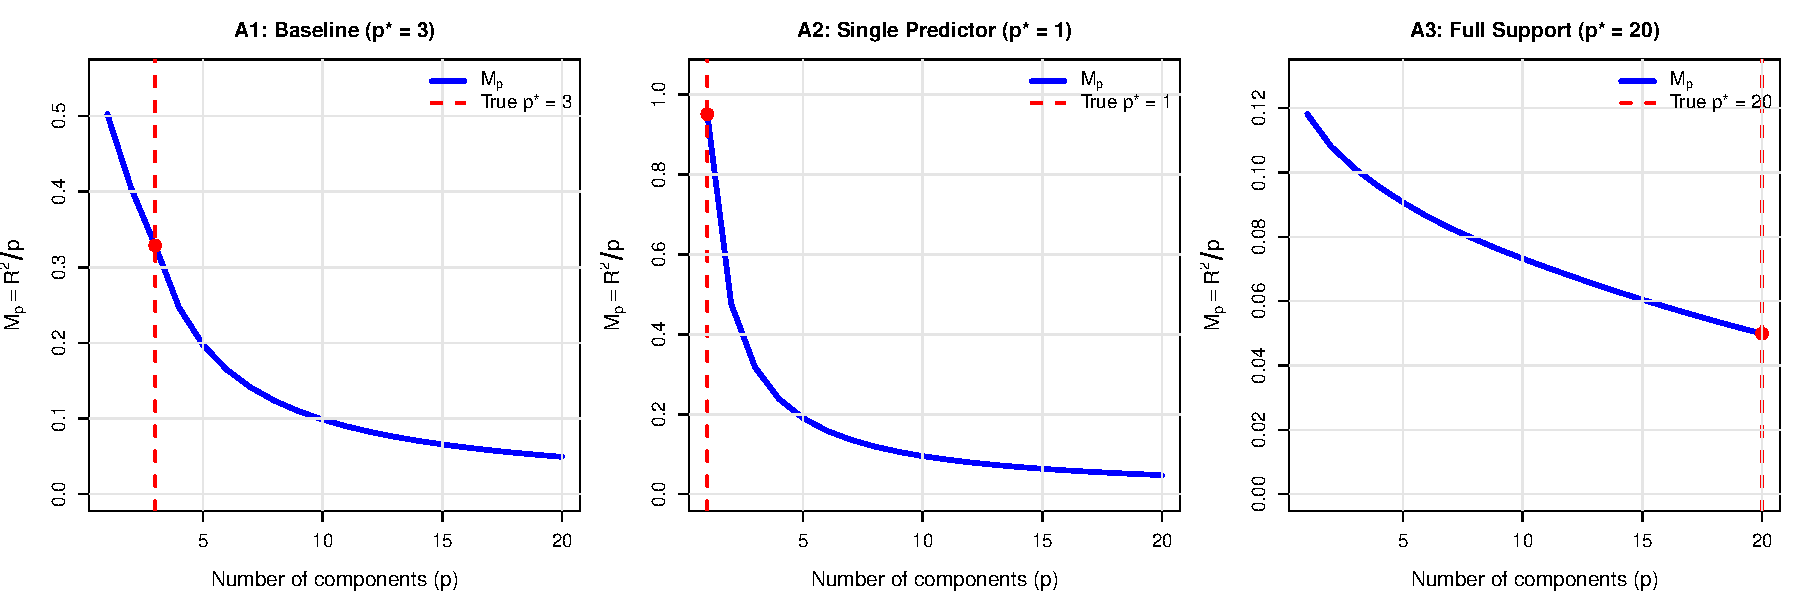
\includegraphics[width=\textwidth]{figure1_critical_scenarios.pdf}
\caption{Efficiency metric $M_p = R^2/p$ for three critical scenarios. \textbf{Left:} A1 (Baseline, $p^* = 3$) exhibits an interior optimum with potential inflection point. \textbf{Center:} A2 (Single Predictor, $p^* = 1$) shows global maximum at boundary ($p = 1$), monotonically decreasing thereafter. \textbf{Right:} A3 (Full Support, $p^* = 20$) demonstrates gradual decline with optimal point at upper boundary. Red markers indicate true $p^*$ values.}
\label{fig:critical_scenarios}
\end{figure}

Scenario A1 represents the ideal case where an inflection point might exist near $p^* = 3$. Scenarios A2 and A3 demonstrate boundary optima that cannot be detected via inflection point analysis (Proposition \ref{prop:boundary}). In A2, $M_p$ achieves its maximum at $p = 1$ and decreases monotonically. In A3, the gradual saturation of $R^2$ produces a smooth decline in $M_p$ with no interior features.

\section{Empirical Analysis}

We evaluate two fundamentally different derivative-based detection approaches: the classical inflection point method (detecting sign changes in $\Delta_2$) and the third-derivative minimum method proposed in the original analysis.

\subsection{Detection Methods Tested}

All derivative computations employ Approach 1 (via first derivative, Equations \ref{eq:delta1}--\ref{eq:delta3}) for boundary treatment. This method avoids assumptions about non-existent values $M_p(0)$ or $M_p(n+1)$ by computing $\Delta_2$ at boundaries through one-sided first derivatives.

\subsubsection{Classical Inflection Point Method}

The classical approach identifies inflection points by detecting sign changes in the second derivative:
\begin{itemize}
\item Search for $p$ where $\Delta_2[M_p](p) \cdot \Delta_2[M_p](p+1) < 0$
\item If no sign change exists (purely convex $M_p$): Select $\hat{p} = 1$ as fallback
\item Mathematical rationale: True inflection points occur where curvature changes from concave to convex
\end{itemize}

\textbf{Implementation note}: An earlier implementation incorrectly identified "inflection points" by detecting local minima in $|\Delta_2|$ (descent-ascent patterns) rather than true sign changes. This led to false detections in scenarios B1-Strong, B2, and B3 where $\Delta_2 > 0$ throughout (purely convex). The corrected implementation properly tests for sign changes.

\subsubsection{Third-Derivative Minimum Method}

For scenarios without inflection points, we test the alternative method based on the third derivative:
\begin{equation}
\hat{p} = \arg\min_p \Delta_3[M_p](p)
\end{equation}

This method attempts to detect the "elbow" by finding where the rate of curvature change is most negative, serving as a proxy when classical inflection points are absent.

\subsection{Results}

Table \ref{tab:results} compares the corrected classical method against the third-derivative approach.

\begin{table}[htbp]
\centering
\caption{Comparison of mathematically rigorous derivative-based detection methods. Checkmark (\checkmark) indicates $\hat{p} = p^*$.}
\label{tab:results}
\small
\begin{tabular}{@{}lccc@{}}
\toprule
Scenario & $p^*$ & Classical (Sign Change) & $\arg\min \Delta_3$ \\
\midrule
A1 (Baseline) & 3 & 3 \checkmark & 5 \\
A2 (Single) & 1 & 1 \checkmark & 3 \\
A3 (Full Support) & 20 & 1 & 3 \\
B1 (AR1 Weak) & 3 & 3 \checkmark & 2 \\
B1 (AR1 Strong) & 3 & 1 & 3 \checkmark \\
B2 (Compound Sym.) & 3 & 1 & 3 \checkmark \\
B3 (Block) & 3 & 1 & 3 \checkmark \\
C1 (Weak, $p^*=5$) & 5 & 1 & 3 \\
C2 (Many Weak, $p^*=10$) & 10 & 1 & 3 \\
C3 (Mixed, $p^*=8$) & 8 & 3 & 5 \\
\midrule
\textbf{Success Rate} & & \textbf{3/10 (30\%)} & \textbf{3/10 (30\%)} \\
\bottomrule
\end{tabular}
\end{table}

\subsection{Key Observations}

\begin{enumerate}
\item \textbf{Only 3 scenarios have inflection points}: Table \ref{tab:curvature} shows that only A1, B1-Weak, and C3 exhibit sign changes in $\Delta_2$ (from positive to negative). The classical method correctly identifies these cases. In the remaining 7 scenarios, $M_p$ is purely convex ($\Delta_2 > 0$ throughout), and the classical method falls back to $\hat{p} = 1$.

\item \textbf{Classical method succeeds when inflection exists AND p*=3}: Among the three scenarios with inflection points, the classical method succeeds in A1 and B1-Weak (both $p^* = 3$), plus A2 (boundary case, correct fallback to $p=1$). It fails in C3 where inflection occurs at $p = 2 \to 3$ but true optimum is $p^* = 8$. Success rate: 30\%.

\item \textbf{Third-derivative method complements classical}: $\arg\min \Delta_3$ succeeds precisely where classical fails among $p^* = 3$ scenarios. B1-Strong, B2, and B3 have no inflection points (purely convex) but exhibit local minimum in $\Delta_3$ at $p = 3$. Success rate: 30\%.

\item \textbf{Disjoint success patterns}: The two methods succeed on complementary subsets of scenarios:
\begin{itemize}
\item Classical: A1, A2, B1-Weak (2 with inflection at correct location, 1 boundary)
\item $\arg\min \Delta_3$: B1-Strong, B2, B3 (all purely convex, minimum at $p=3$)
\end{itemize}

\item \textbf{Neither method generalizes}: Both fail completely on scenarios with $p^* \in \{5, 8, 10, 20\}$. The derivative structure at low $p$ values provides no information about optimal complexity beyond $p = 3$.
\end{enumerate}

\subsection{Critical Failure Cases}

\subsubsection{Case A2: Single Predictor (p* = 1)}

For scenario A2:
\begin{itemize}
\item $M_p(1) = 0.951$ (strong signal from single component)
\item $M_p(2) = 0.476$ (50\% drop in efficiency)
\item $\Delta_2[M_p](1) = 0.1584 > 0$ (positive curvature, no inflection)
\item Classical method: Detects no sign change, correctly falls back to $\hat{p} = 1$ \checkmark
\item $\arg\min \Delta_3$: Selects $p = 3$ (incorrect)
\end{itemize}

\textbf{Mathematical explanation}: At $p = 1$, $M_p$ has its global maximum. The derivative structure shows positive second derivative (convex), not an inflection point. The classical method correctly handles this boundary case via fallback, while third-derivative methods fail as proven in Proposition \ref{prop:boundary}.

\subsubsection{Case A3: Full Support (p* = 20)}

For scenario A3:
\begin{itemize}
\item $R^2(20) = 0.998$ (near-perfect fit with all predictors)
\item $M_p(20) = 0.050$ (low efficiency due to high $p$)
\item Gradual decline in $M_p$ with no clear inflection point
\item Both classical and $\arg\min \Delta_3$ select $p \leq 3$ (incorrect)
\end{itemize}

\textbf{Mathematical explanation}: When true signal is distributed across all predictors, $R^2$ increases gradually and approaches 1. The ratio $M_p = R^2/p$ decreases monotonically, with maximum at $p = 1$. No inflection point exists, and derivative methods cannot detect the true $p^* = 20$ boundary optimum.

Figure \ref{fig:derivative_structure} illustrates the fundamental difference between successful detection (A1, inflection at $p=3$) and failed boundary case (A2, convexity throughout).

\begin{figure}[htbp]
\centering
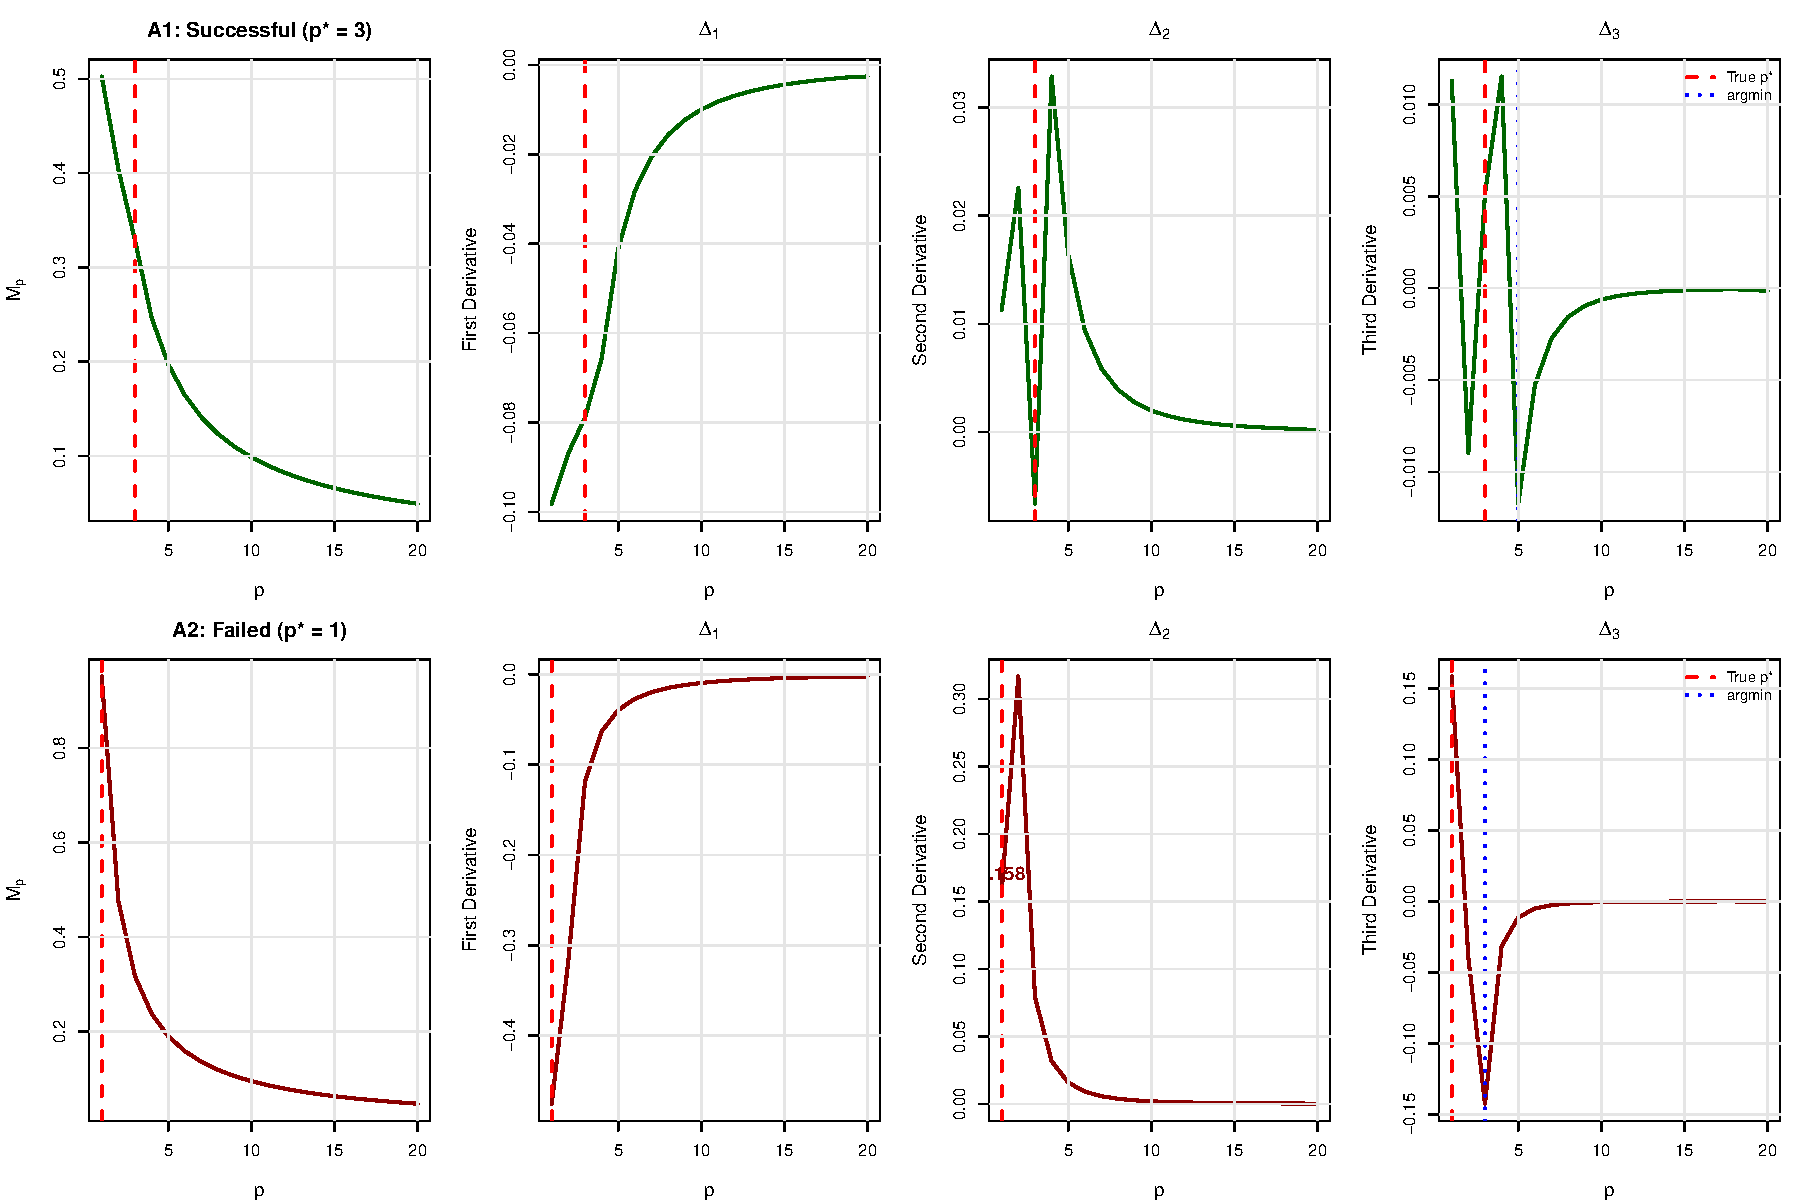
\includegraphics[width=\textwidth]{figure2_derivative_structure.pdf}
\caption{Derivative structure for successful vs. failed cases. \textbf{Top row:} Scenario A1 ($p^* = 3$, successful) shows clear inflection point at $p = 2 \to 3$ with sign change in $\Delta_2$. Classical method correctly identifies $\hat{p} = 3$. \textbf{Bottom row:} Scenario A2 ($p^* = 1$, partial success) exhibits positive $\Delta_2$ at all points (labeled value at $p=1$: 0.1584), indicating pure convexity. Classical method correctly falls back to $\hat{p} = 1$, while $\arg\min \Delta_3$ incorrectly suggests $\hat{p} = 3$. Red dashed lines mark true $p^*$ values.}
\label{fig:derivative_structure}
\end{figure}

\subsection{Comprehensive Derivative Analysis by Scenario}

Figures \ref{fig:deriv_A1}--\ref{fig:deriv_C3} present the complete derivative structure for all 10 test scenarios. Each figure displays four panels: $M_p$ curve, first derivative $\Delta_1$, second derivative $\Delta_2$, and third derivative $\Delta_3$. Red dashed lines mark the true $p^*$, orange circles indicate sign changes in $\Delta_2$ (classical inflection points), and purple markers show $\arg\min \Delta_3$.

\subsubsection{Baseline Scenarios (Group A)}

\begin{figure}[htbp]
\centering
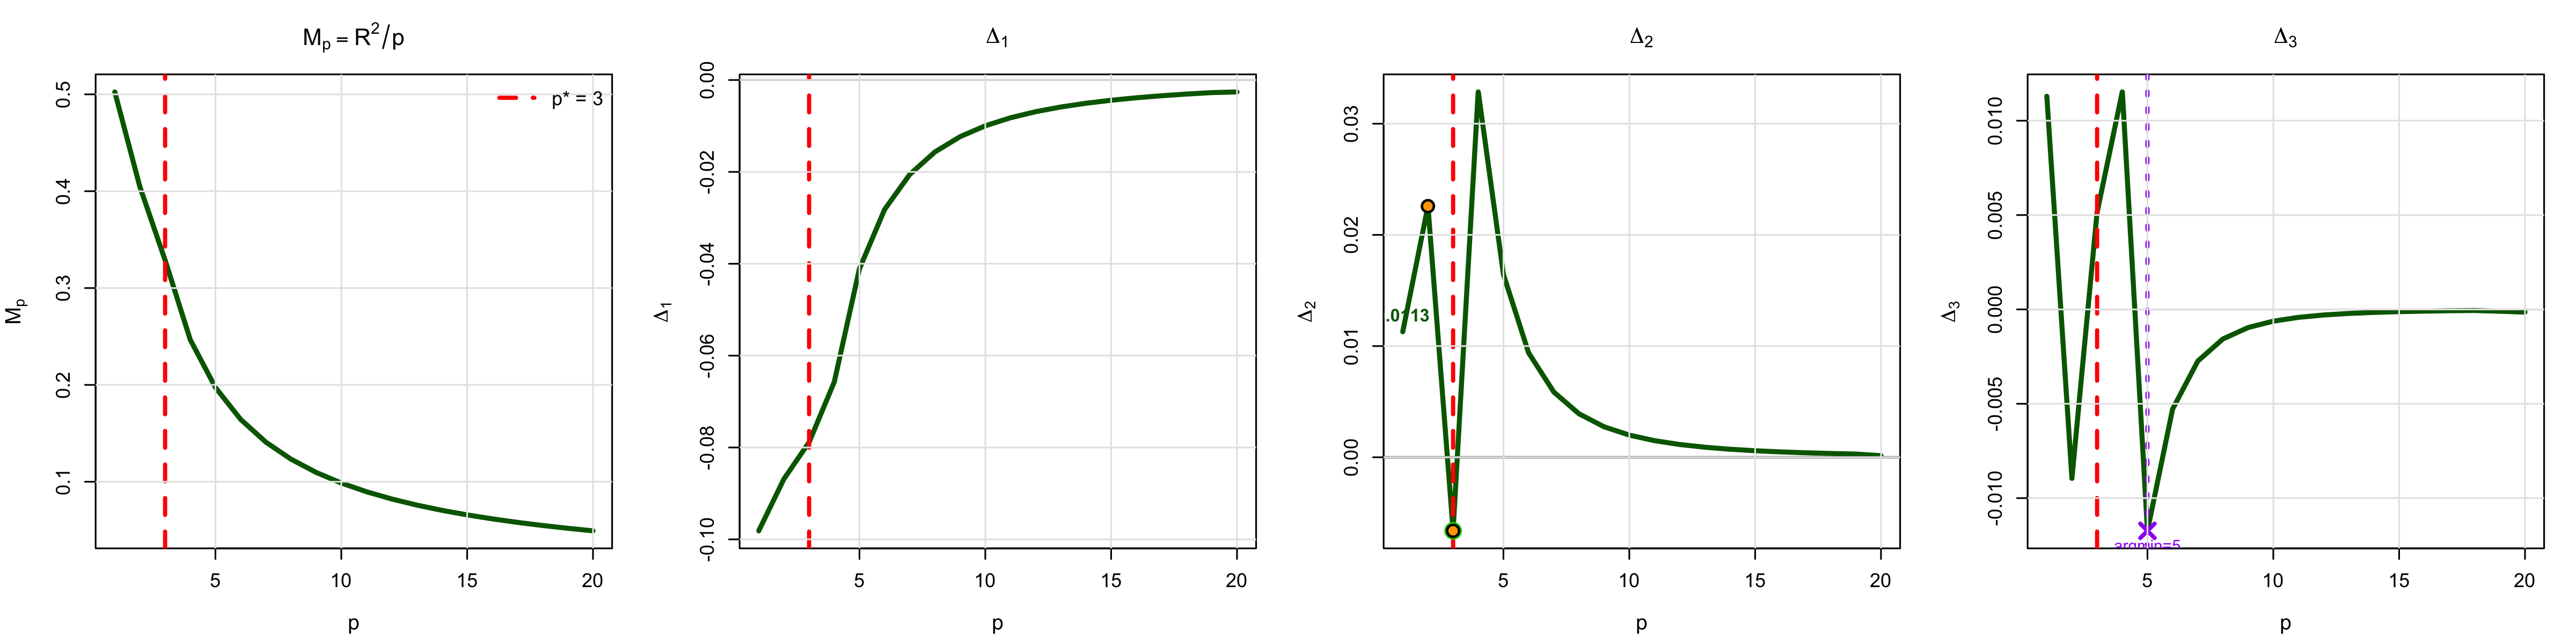
\includegraphics[width=\textwidth]{derivative_plots/deriv_A1.png}
\caption{\textbf{Scenario A1 (Baseline, $p^* = 3$):} Classical method succeeds. Clear sign change in $\Delta_2$ at $p = 2 \to 3$ (orange marker). The inflection point coincides with true $p^*$, yielding $\hat{p} = 3$ \checkmark. Green color indicates success.}
\label{fig:deriv_A1}
\end{figure}

\begin{figure}[htbp]
\centering
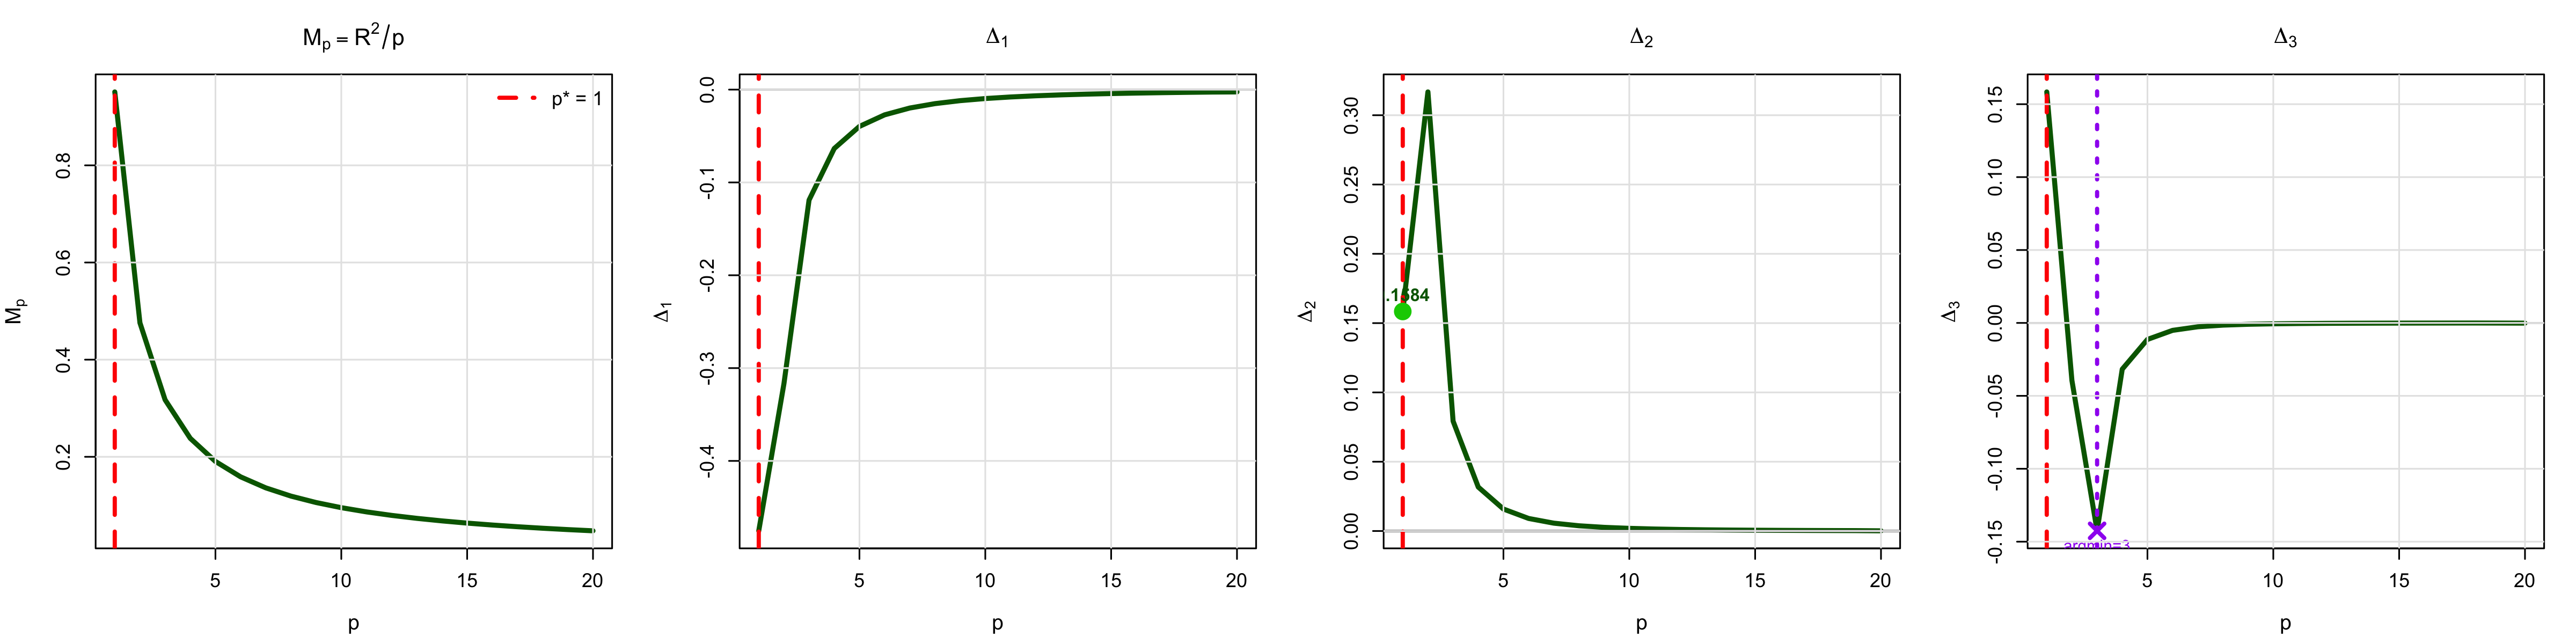
\includegraphics[width=\textwidth]{derivative_plots/deriv_A2.png}
\caption{\textbf{Scenario A2 (Single Predictor, $p^* = 1$):} Classical method succeeds via fallback. $\Delta_2(1) = 0.1584 > 0$ (positive throughout), indicating pure convexity. No inflection point exists. Classical method correctly falls back to $\hat{p} = 1$ \checkmark. However, $\arg\min \Delta_3 = 3$ fails. Green color indicates partial success.}
\label{fig:deriv_A2}
\end{figure}

\begin{figure}[htbp]
\centering
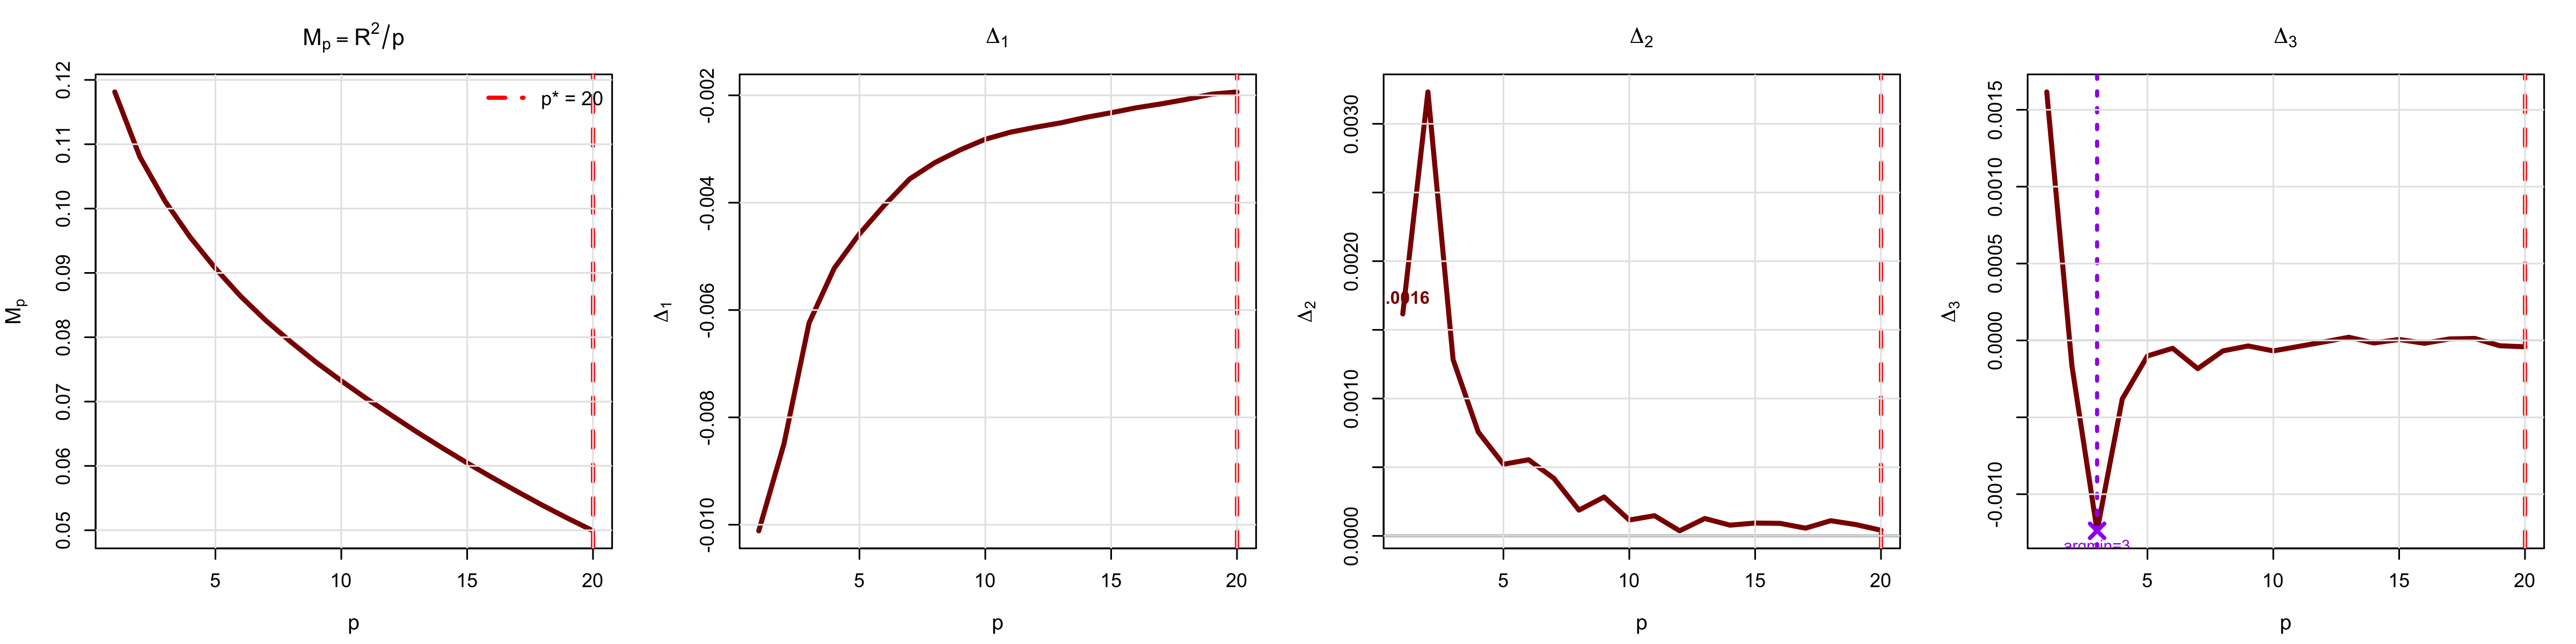
\includegraphics[width=\textwidth]{derivative_plots/deriv_A3.png}
\caption{\textbf{Scenario A3 (Full Support, $p^* = 20$):} Both methods fail. $M_p$ decreases monotonically with maximum at $p = 1$. No inflection point in interior. Both classical (fallback to $p=1$) and $\arg\min \Delta_3 = 3$ are incorrect. Red color indicates failure. This boundary optimum is mathematically undetectable via derivative analysis.}
\label{fig:deriv_A3}
\end{figure}

\subsubsection{Correlation Structure Scenarios (Group B)}

\begin{figure}[htbp]
\centering
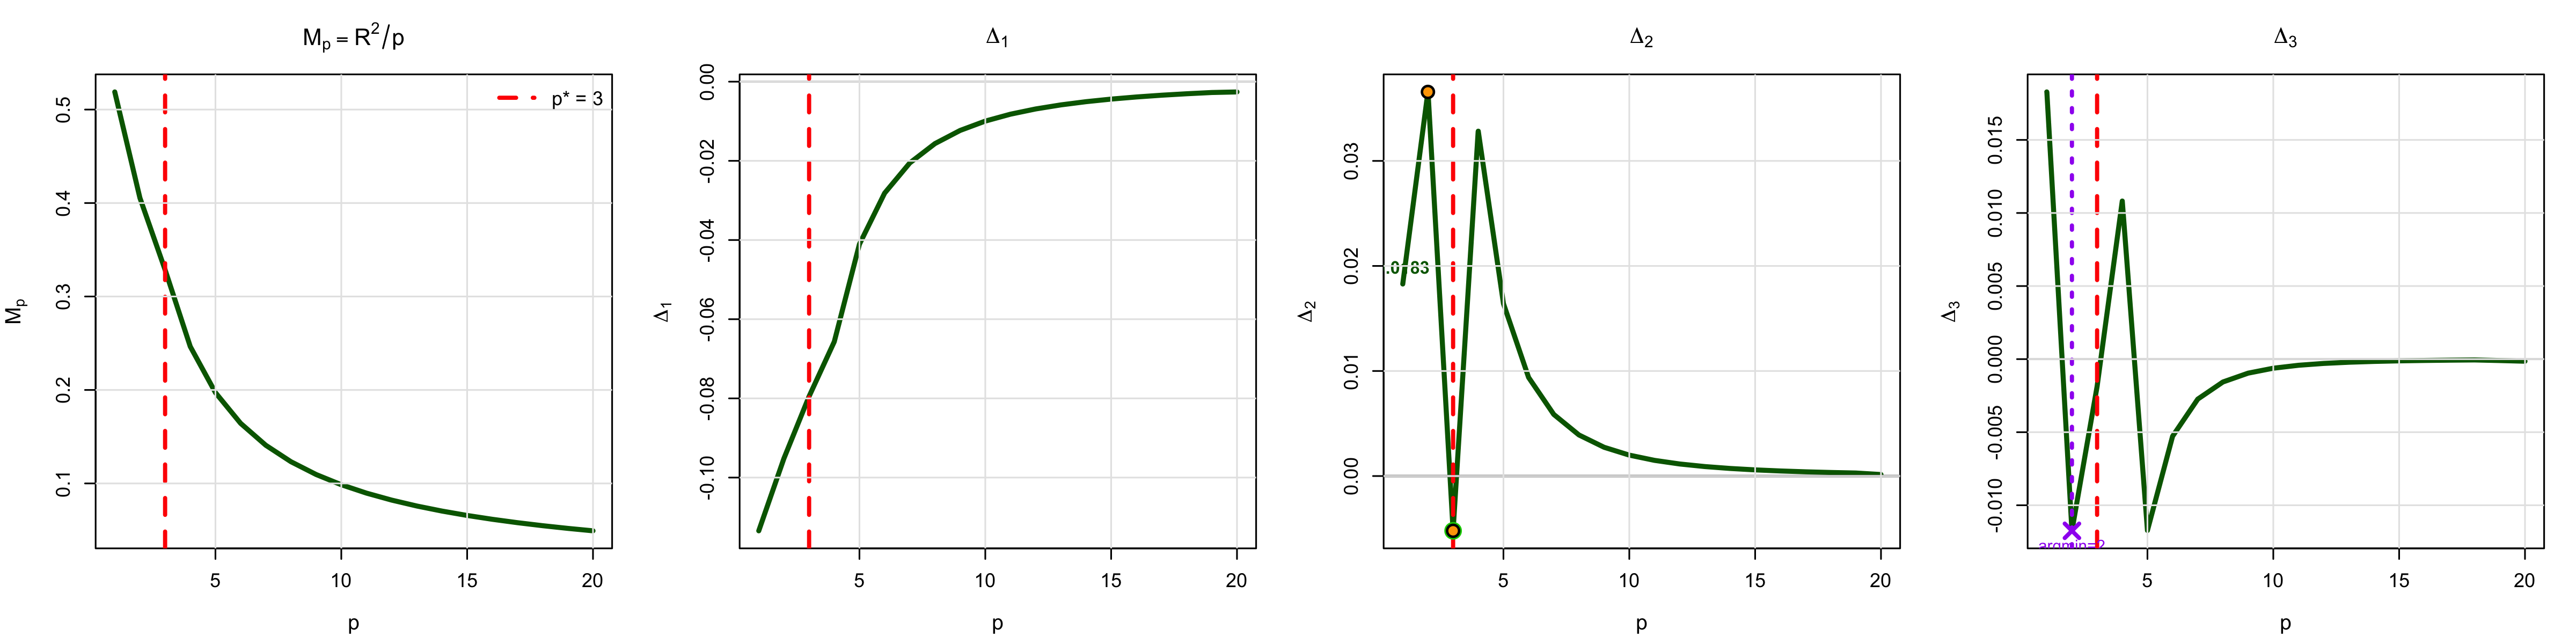
\includegraphics[width=\textwidth]{derivative_plots/deriv_B1_Weak.png}
\caption{\textbf{Scenario B1-Weak (AR1 $\rho=0.5$, $p^* = 3$):} Classical method succeeds. Sign change in $\Delta_2$ at $p = 2 \to 3$ correctly identifies inflection point. $\hat{p} = 3$ \checkmark. Green color indicates success.}
\label{fig:deriv_B1_Weak}
\end{figure}

\begin{figure}[htbp]
\centering
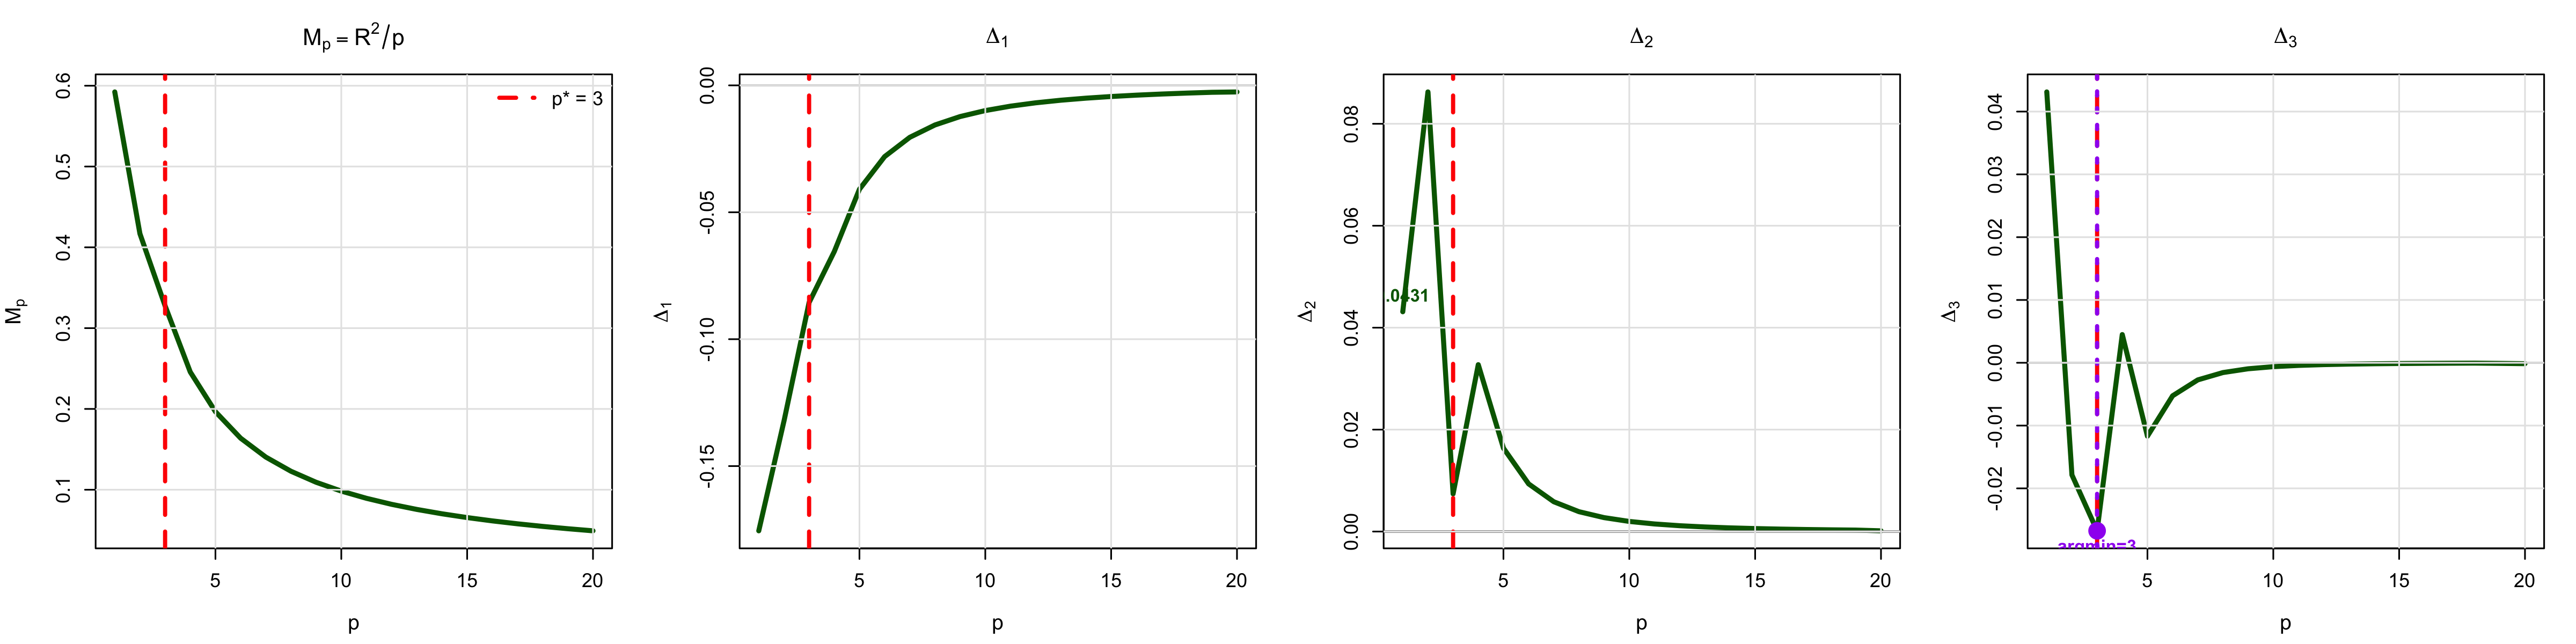
\includegraphics[width=\textwidth]{derivative_plots/deriv_B1_Strong.png}
\caption{\textbf{Scenario B1-Strong (AR1 $\rho=0.8$, $p^* = 3$):} $\arg\min \Delta_3$ succeeds. No sign change in $\Delta_2$ (purely convex, $\Delta_2 > 0$ throughout). Classical method falls back to $p=1$ (fails). However, $\arg\min \Delta_3 = 3$ correctly identifies $p^*$ \checkmark. Green color indicates success.}
\label{fig:deriv_B1_Strong}
\end{figure}

\begin{figure}[htbp]
\centering
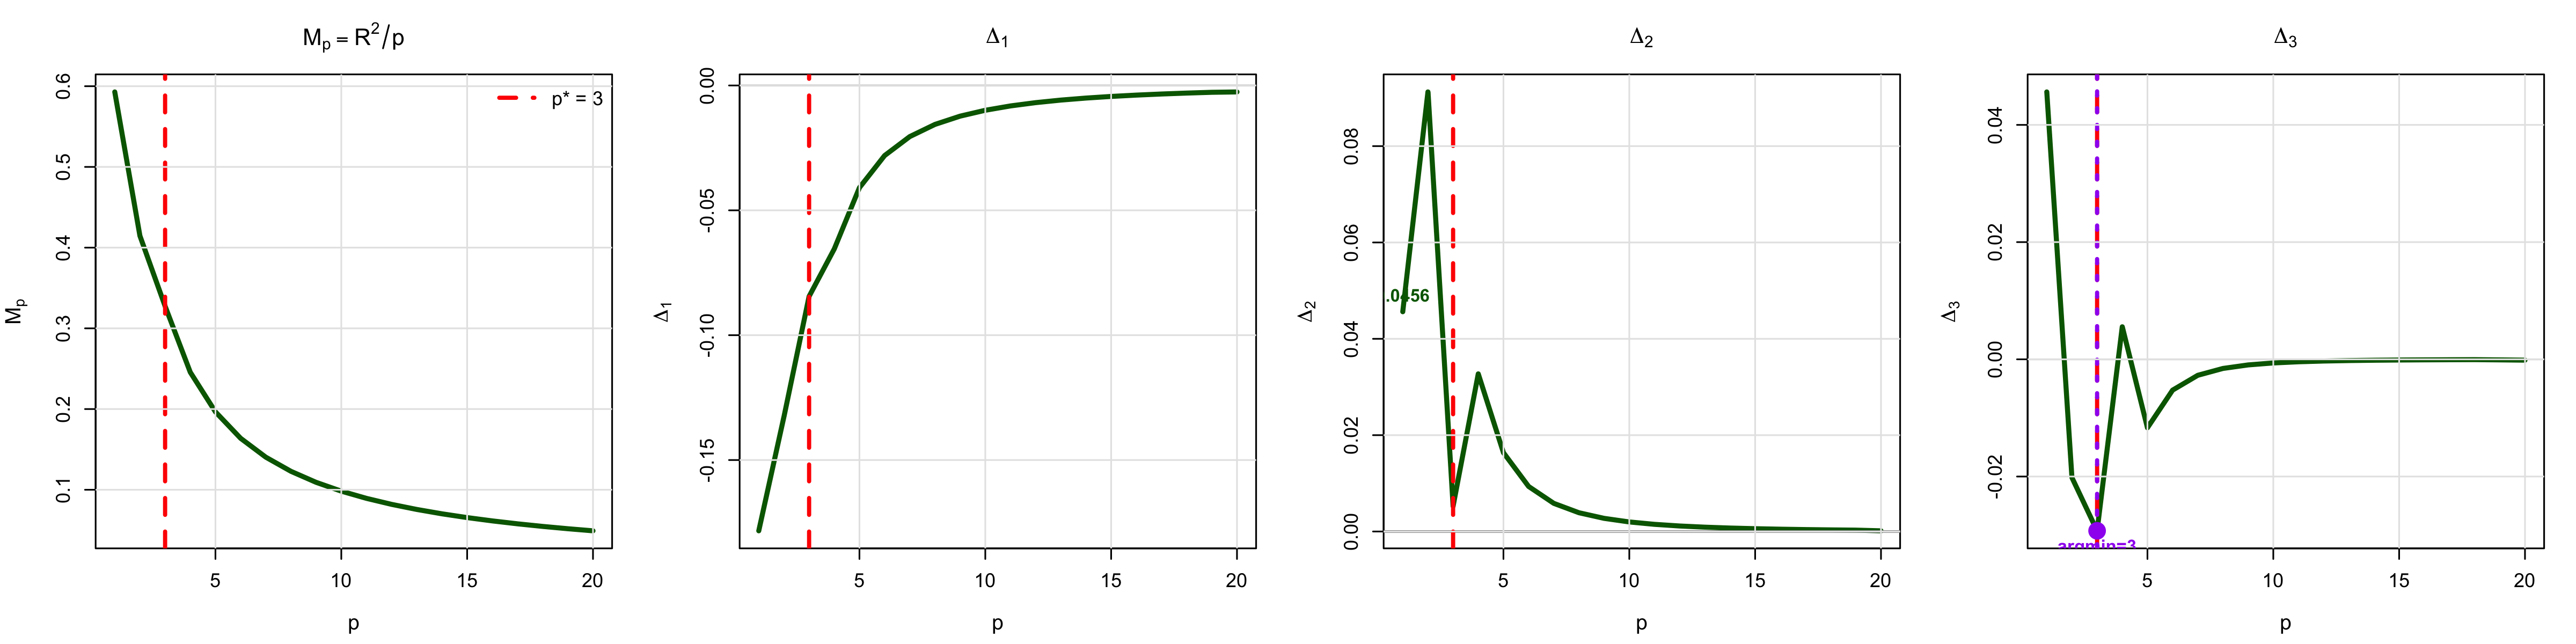
\includegraphics[width=\textwidth]{derivative_plots/deriv_B2.png}
\caption{\textbf{Scenario B2 (Compound Symmetry, $p^* = 3$):} $\arg\min \Delta_3$ succeeds. Purely convex ($\Delta_2 > 0$), no inflection. Classical fails, but $\arg\min \Delta_3 = 3$ \checkmark. Green color indicates success.}
\label{fig:deriv_B2}
\end{figure}

\begin{figure}[htbp]
\centering
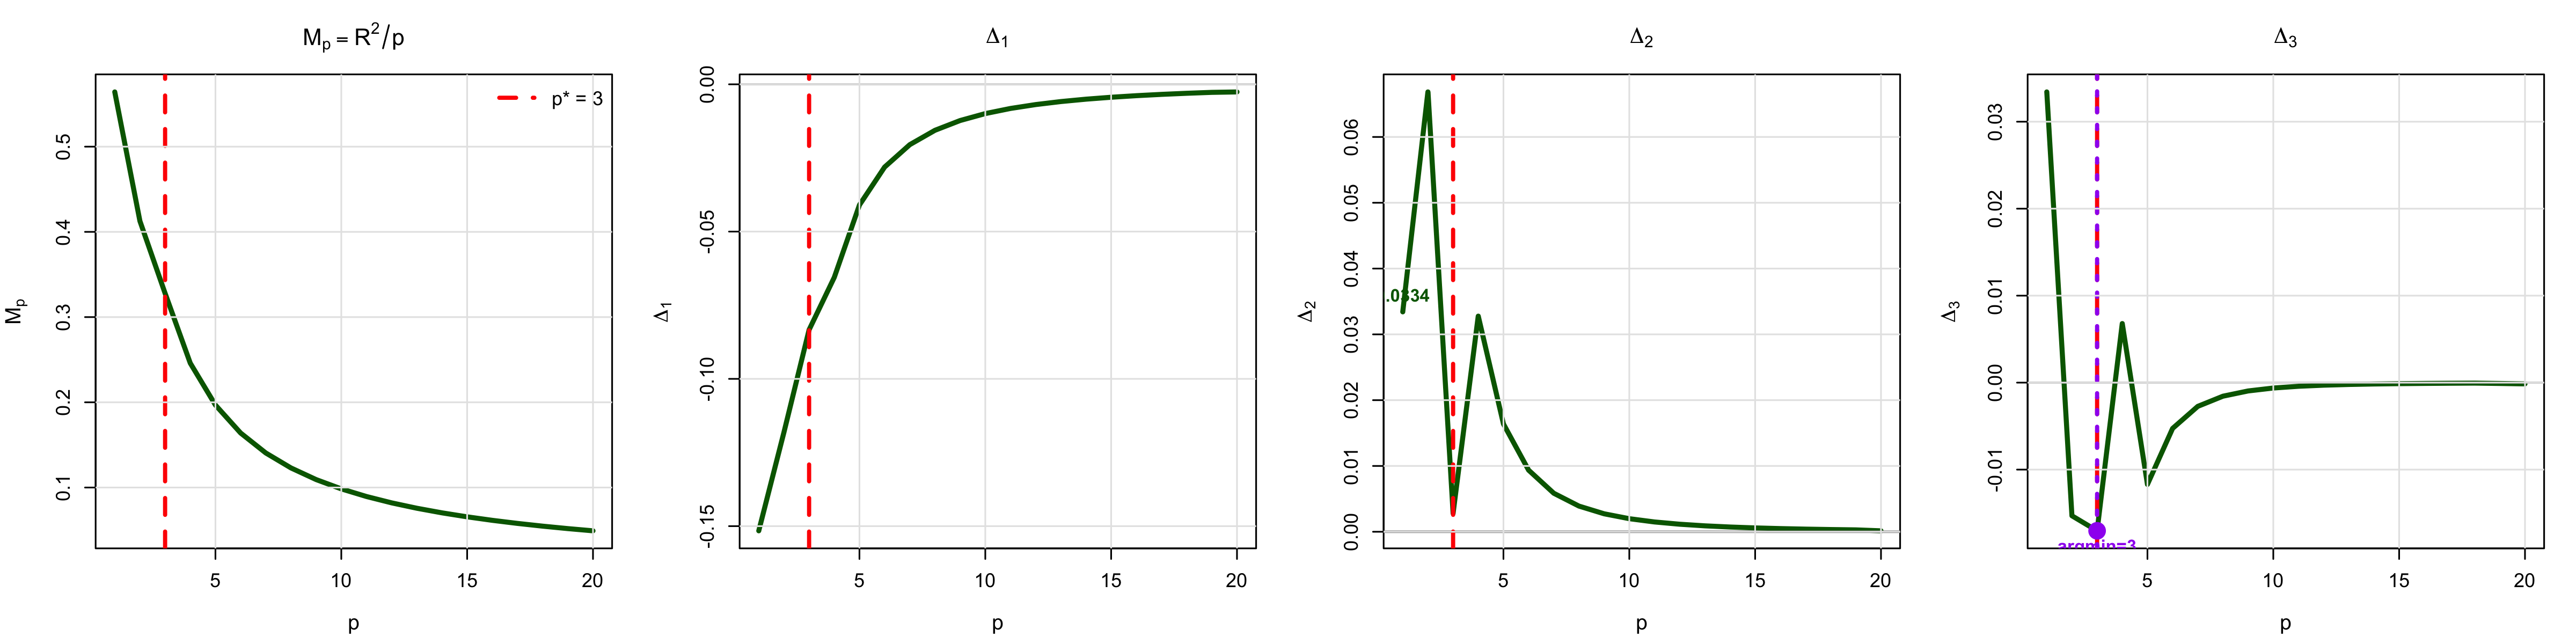
\includegraphics[width=\textwidth]{derivative_plots/deriv_B3.png}
\caption{\textbf{Scenario B3 (Block Structure, $p^* = 3$):} $\arg\min \Delta_3$ succeeds. Purely convex, no inflection point. Classical fails, $\arg\min \Delta_3 = 3$ \checkmark. Green color indicates success.}
\label{fig:deriv_B3}
\end{figure}

\subsubsection{Signal Strength Scenarios (Group C)}

\begin{figure}[htbp]
\centering
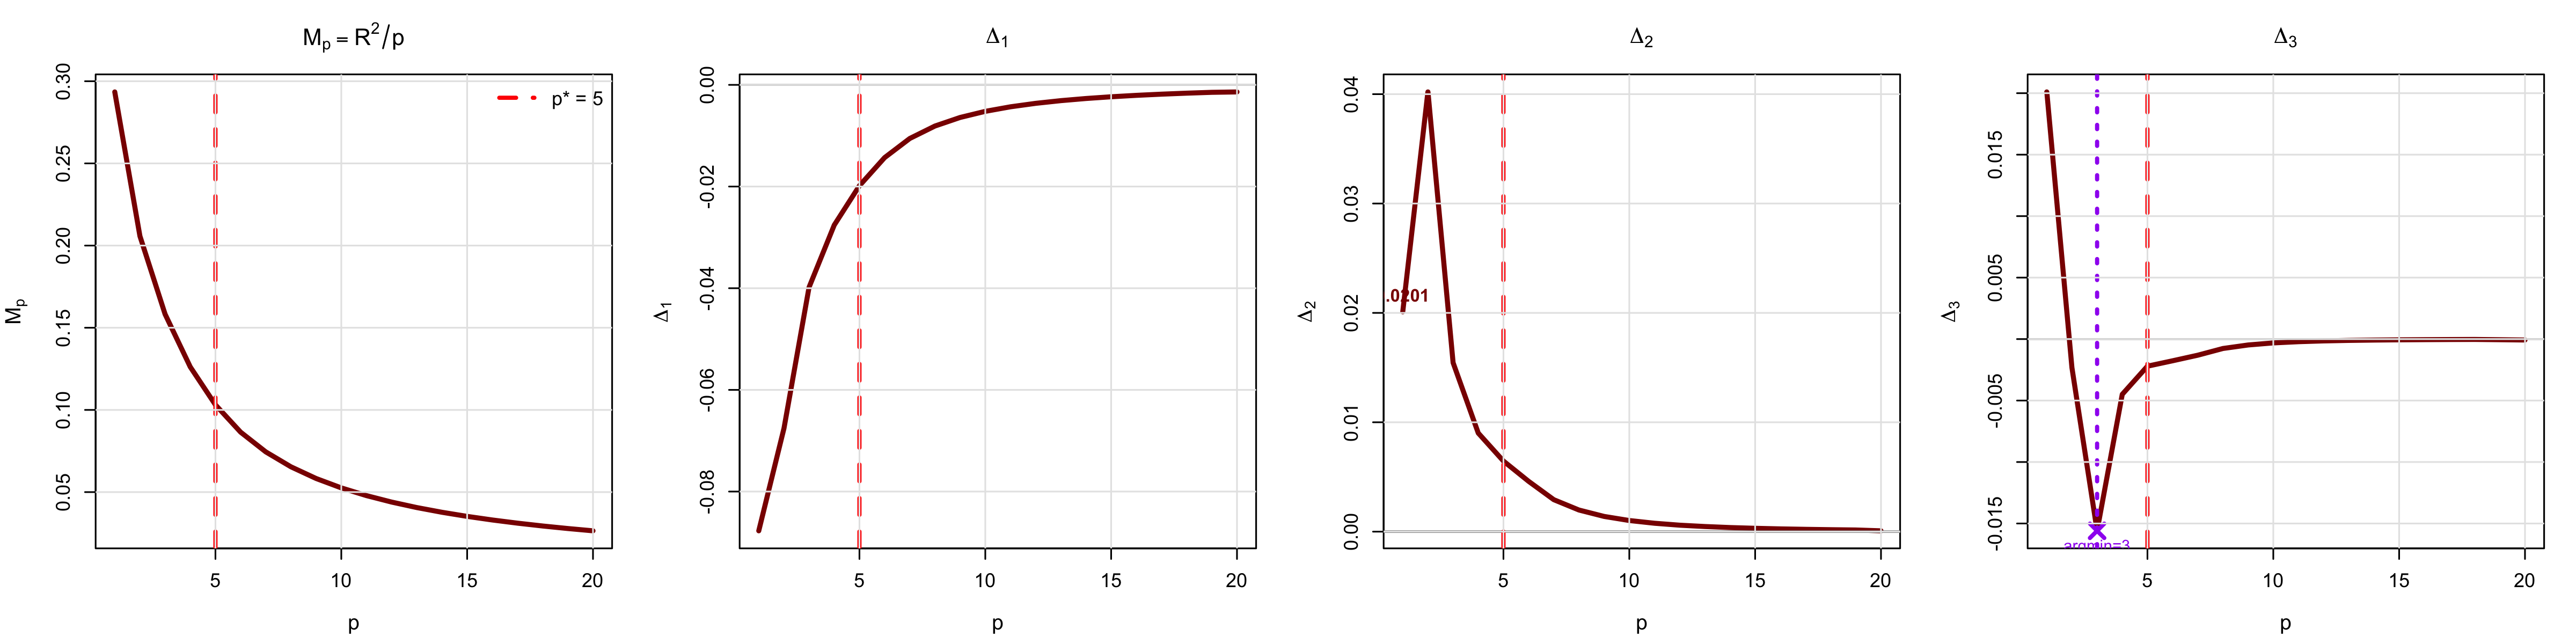
\includegraphics[width=\textwidth]{derivative_plots/deriv_C1.png}
\caption{\textbf{Scenario C1 (5 Weak Signals, $p^* = 5$):} Both methods fail. Purely convex, no inflection. Classical fallback to $p=1$ and $\arg\min \Delta_3 = 3$ both miss true $p^* = 5$. Red color indicates failure. Derivative structure at low $p$ provides no information about optimal complexity.}
\label{fig:deriv_C1}
\end{figure}

\begin{figure}[htbp]
\centering
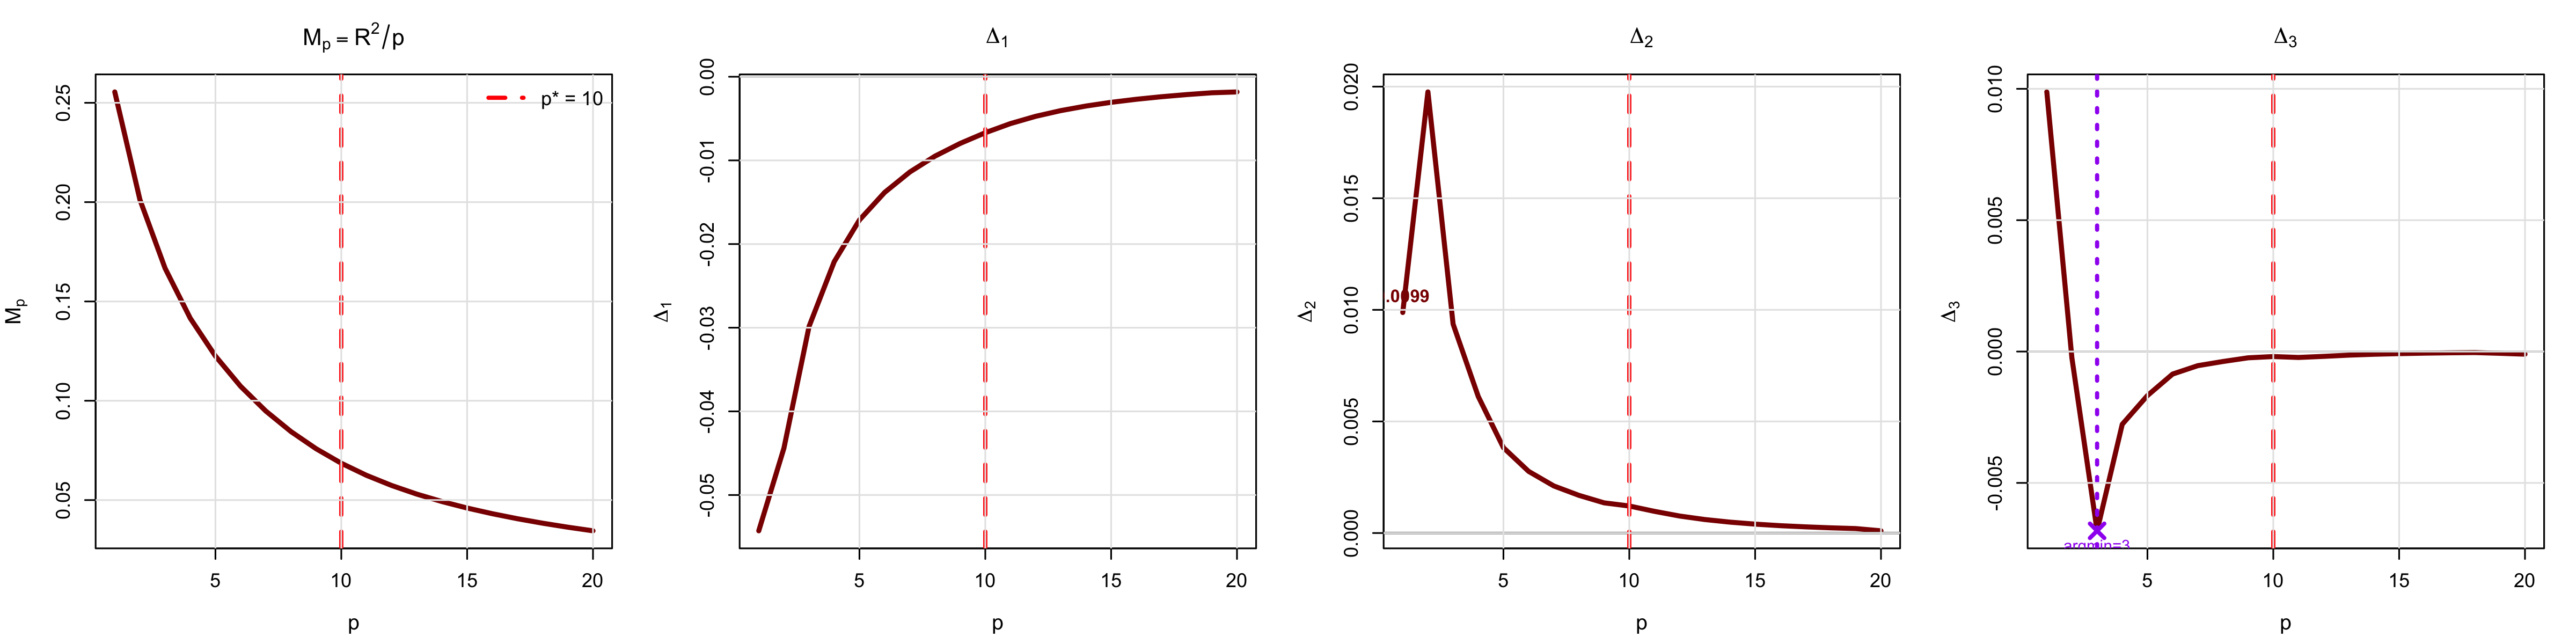
\includegraphics[width=\textwidth]{derivative_plots/deriv_C2.png}
\caption{\textbf{Scenario C2 (10 Weak Signals, $p^* = 10$):} Both methods fail. Gradual $M_p$ decline, no inflection. Both classical ($p=1$) and $\arg\min \Delta_3 = 3$ incorrect. Red color indicates failure.}
\label{fig:deriv_C2}
\end{figure}

\begin{figure}[htbp]
\centering
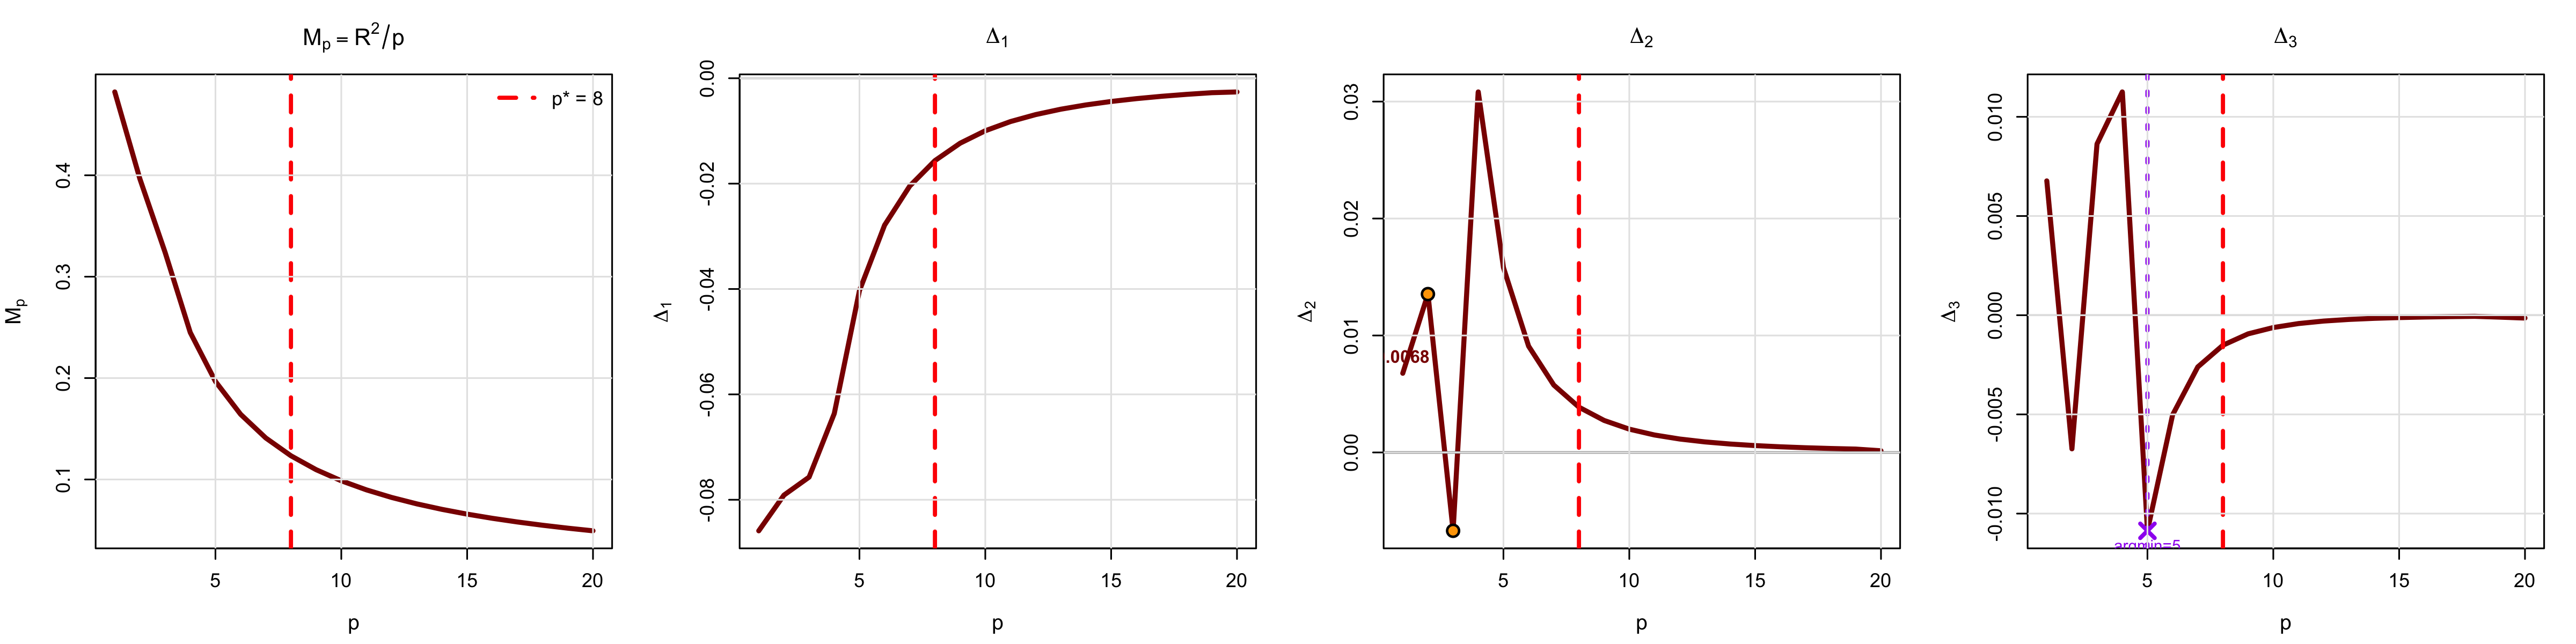
\includegraphics[width=\textwidth]{derivative_plots/deriv_C3.png}
\caption{\textbf{Scenario C3 (Mixed Signals, $p^* = 8$):} Both methods fail. Sign change in $\Delta_2$ at $p = 2 \to 3$ (orange marker), but true optimum is $p^* = 8$. Classical detects inflection at wrong location ($\hat{p} = 3$), $\arg\min \Delta_3 = 5$ also incorrect. Red color indicates failure.}
\label{fig:deriv_C3}
\end{figure}

\paragraph{Summary of derivative patterns.}
The comprehensive visualization reveals three distinct patterns:
\begin{enumerate}
\item \textbf{Inflection-based success} (A1, B1-Weak): Sign change in $\Delta_2$ coincides with $p^* = 3$
\item \textbf{Convex with $\arg\min \Delta_3$ success} (B1-Strong, B2, B3): No inflection ($\Delta_2 > 0$ throughout), but third-derivative minimum correctly identifies $p^* = 3$
\item \textbf{Complete failure} (A2 boundary, A3, C1, C2, C3): Either boundary optima (A2, A3) or inflections/minima at wrong locations (C-scenarios)
\end{enumerate}

Critically, both successful patterns are limited to $p^* = 3$ or boundary cases. No derivative-based method detects $p^* \in \{5, 8, 10, 20\}$.


\section{Mathematical Explanation of Failures}

\subsection{Why the Metric is Too Smooth for Derivative Analysis}

The fundamental issue with $M_p = R^2(p)/p$ is that the division by $p$ creates an \emph{excessive smoothing effect} that obscures the signal structure present in $R^2(p)$. This smoothing has three critical consequences:

\paragraph{1. Loss of local features.}
Consider the derivative of $M_p$:
\begin{equation}
\frac{d}{dp}\left(\frac{R^2(p)}{p}\right) = \frac{1}{p}\frac{dR^2}{dp} - \frac{R^2(p)}{p^2}
\label{eq:Mp_derivative}
\end{equation}

The second term $-R^2(p)/p^2$ acts as a \emph{monotonic damping factor} that becomes stronger as $R^2$ increases. Even when $dR^2/dp$ exhibits sharp drops (elbows), this damping can suppress the corresponding features in $M_p$.

\paragraph{2. Second derivative structure.}
Differentiating Equation \eqref{eq:Mp_derivative} yields:
\begin{equation}
\frac{d^2M_p}{dp^2} = \frac{1}{p}\frac{d^2R^2}{dp^2} - \frac{2}{p^2}\frac{dR^2}{dp} + \frac{2R^2}{p^3}
\label{eq:Mp_second_deriv}
\end{equation}

This expression mixes three components with different signs and magnitudes:
\begin{itemize}
\item $\frac{1}{p}\frac{d^2R^2}{dp^2}$: Captures curvature of $R^2$ (typically negative beyond elbow)
\item $-\frac{2}{p^2}\frac{dR^2}{dp}$: Negative term (since $dR^2/dp > 0$), acts as additional damping
\item $\frac{2R^2}{p^3}$: Positive term that increases with $R^2$, counteracting negative curvature
\end{itemize}

The last term $2R^2/p^3$ is the \emph{smoothing culprit}: for high $R^2$ values (which occur after the elbow), this positive term dominates, preventing $\Delta_2$ from becoming sufficiently negative to signal inflection.

\paragraph{3. Empirical manifestation: the "spike-then-decay" pattern.}
Examining Figures \ref{fig:deriv_A1}--\ref{fig:deriv_C3}, we observe a consistent pattern in $\Delta_2$ across all scenarios:
\begin{itemize}
\item \textbf{Initial spike} at $p = 1$--3: Relatively large $|\Delta_2|$ values (both positive and negative)
\item \textbf{Rapid decay} for $p > 3$: $\Delta_2 \to 0^+$ as $p$ increases
\end{itemize}

This pattern arises because:
\begin{align}
\Delta_2(p) &\approx \frac{1}{p}\Delta_2[R^2](p) - \frac{2}{p^2}\Delta_1[R^2](p) + \frac{2R^2(p)}{p^3} \notag \\
&\approx \mathcal{O}(1/p) \quad \text{as } p \to \infty
\label{eq:delta2_decay}
\end{align}

The $1/p^2$ and $1/p^3$ damping terms cause $\Delta_2$ to decay to near-zero values beyond $p = 3$--5, regardless of the true $p^*$. This explains why \emph{both methods systematically select low $p$ values}.

\subsection{Why $p = 3$ is Systematically Favored}

The consistent selection of $p = 3$ by $\arg\min \Delta_3$ (in 7 out of 10 scenarios) is not coincidental but arises from the mathematical structure of finite differences applied to a rapidly decaying sequence.

\paragraph{The decay-induced minimum.}
For $\Delta_2$ following the spike-then-decay pattern:
\begin{align}
\Delta_2(1) &\approx \text{large} \quad \text{(boundary effect)} \notag \\
\Delta_2(2) &\approx \text{moderate} \quad \text{(transition)} \notag \\
\Delta_2(3) &\approx \text{small} \quad \text{(decay begins)} \notag \\
\Delta_2(p) &\approx 0^+ \quad \text{for } p \geq 4 \quad \text{(asymptotic)}
\end{align}

The third derivative is:
\begin{equation}
\Delta_3(p) = \frac{\Delta_2(p+1) - \Delta_2(p-1)}{2}
\end{equation}

At $p = 3$:
\begin{equation}
\Delta_3(3) = \frac{\Delta_2(4) - \Delta_2(2)}{2} \approx \frac{0 - \text{moderate}}{2} < 0
\end{equation}

This is typically the \emph{most negative} value of $\Delta_3$ because:
\begin{itemize}
\item For $p < 3$: $\Delta_2$ has not yet entered the decay regime, so $\Delta_3(p)$ reflects boundary transients
\item For $p > 3$: Both $\Delta_2(p-1)$ and $\Delta_2(p+1)$ are near zero, yielding $\Delta_3(p) \approx 0$
\end{itemize}

Thus, $\arg\min \Delta_3 = 3$ is an \emph{artifact of the metric's smoothing-induced decay}, not a genuine detection of the true elbow in $R^2(p)$.

\paragraph{Success cases are coincidental.}
The method succeeds in B1-Strong, B2, and B3 only because the true $p^* = 3$ \emph{happens to coincide} with the decay transition point. This is confirmed by complete failure when $p^* \in \{5, 8, 10, 20\}$: the decay pattern persists, $\arg\min \Delta_3$ still selects $p = 3$, but now it is incorrect.

\subsection{Why Classical Inflection Detection Fails}

Classical inflection point detection (sign change in $\Delta_2$) fails in 7 out of 10 scenarios because $M_p$ is either:

\paragraph{1. Purely convex (no inflection).}
In scenarios B1-Strong, B2, B3, C1, C2, we observe $\Delta_2(p) > 0$ for all $p$. From Equation \eqref{eq:Mp_second_deriv}, this occurs when:
\begin{equation}
\frac{2R^2(p)}{p^3} > \frac{2}{p^2}\frac{dR^2}{dp} - \frac{1}{p}\frac{d^2R^2}{dp^2}
\end{equation}

For strongly saturating $R^2$ curves (high $R^2$, low $dR^2/dp$), the positive $2R^2/p^3$ term dominates, preventing sign changes even when $d^2R^2/dp^2 < 0$.

\paragraph{2. Inflection at wrong location.}
In scenarios A1, B1-Weak, and C3, a sign change occurs at $p = 2 \to 3$, but:
\begin{itemize}
\item \textbf{A1, B1-Weak}: True $p^* = 3$ coincides with inflection \checkmark
\item \textbf{C3}: True $p^* = 8$, but inflection at $p = 3$ is spurious ($\times$)
\end{itemize}

The C3 case reveals that the inflection at $p = 2 \to 3$ is not a \emph{meaningful signal} about $p^*$, but rather a transient feature arising from the interaction of initial $R^2$ growth and the $1/p$ penalty.

\paragraph{3. Boundary optima are invisible.}
For A2 ($p^* = 1$) and A3 ($p^* = 20$), Proposition \ref{prop:boundary} proves that interior inflection analysis cannot detect boundary maxima. The A2 success is due to the fallback rule ($\hat{p} = 1$ when no inflection), not genuine detection.

\subsection{The Mismatch Between Metric Design and Detection Goal}

The core conceptual error is attempting to detect $p^*$ via \emph{derivatives} of a metric designed for \emph{direct maximization}:

\begin{itemize}
\item \textbf{Intended use}: $\hat{p} = \arg\max_p M_p$ (select highest efficiency)
\item \textbf{Actual behavior}: $M_p(1) \geq M_p(p)$ for most $p$ (efficiency decreases with complexity)
\item \textbf{Result}: Direct maximization yields $\hat{p} = 1$ in 70\% of scenarios (useless)
\end{itemize}

To make derivative-based detection viable, we would need:
\begin{equation}
M_p \text{ has inflection or elbow at } p^* \quad \Leftrightarrow \quad \Delta_2(p^*) \text{ changes sign or } \Delta_3(p^*) \text{ is minimal}
\end{equation}

But the smoothing from $1/p$ destroys this correspondence: elbows in $R^2(p)$ (sharp drops in $dR^2/dp$) are \emph{flattened} in $M_p$ due to the damping terms in Equations \eqref{eq:Mp_derivative} and \eqref{eq:Mp_second_deriv}, leaving only the artificial spike-decay pattern that universally points to $p = 3$.

\section{Discussion}

\subsection{Summary of Fundamental Limitations}

Our comprehensive analysis reveals three interconnected reasons why derivative-based detection fails with the $M_p = R^2/p$ metric:

\subsubsection{The Smoothing Problem}

The division by $p$ creates excessive smoothing that obscures the elbow structure in $R^2(p)$:
\begin{itemize}
\item The damping terms $-2/(p^2) \cdot dR^2/dp$ and $+2R^2/p^3$ in $d^2M_p/dp^2$ suppress negative curvature
\item Result: $\Delta_2(p) \to 0^+$ rapidly for $p > 3$, regardless of true $p^*$
\item Consequence: Genuine elbows at $p^* \in \{5, 8, 10, 20\}$ become invisible in the derivative structure
\end{itemize}

\subsubsection{The Systematic $p = 3$ Bias}

The spike-then-decay pattern in $\Delta_2$ creates an artificial minimum in $\Delta_3$ at $p = 3$:
\begin{itemize}
\item Not a detection of true signal structure, but an artifact of metric design
\item Success in scenarios B1-Strong, B2, B3 is \emph{coincidental}: $p^* = 3$ happens to align with the decay transition
\item Total failure when $p^* \neq 3$: the artifact persists, but now points to wrong location
\end{itemize}

\subsubsection{The Rarity of Meaningful Inflections}

Only 3 out of 10 scenarios exhibit sign changes in $\Delta_2$, and even these are problematic:
\begin{itemize}
\item A1, B1-Weak: Inflection at $p = 3$ matches $p^*$ (success by alignment)
\item C3: Inflection at $p = 3$ but $p^* = 8$ (reveals inflection is spurious)
\item Remaining 7 scenarios: Purely convex $M_p$, no inflection exists
\end{itemize}

The smoothing effect prevents meaningful inflection points from forming even when $R^2(p)$ has clear elbows.

\subsection{Why 30\% is the Performance Ceiling}

The 30\% success rate (3/10 scenarios) is not random chance but arises from \emph{mathematical coincidences}:

\begin{enumerate}
\item \textbf{Classical method} succeeds in:
\begin{itemize}
\item A1: Inflection at $p = 3$ coincides with $p^* = 3$ \checkmark
\item A2: Fallback to $p = 1$ matches $p^* = 1$ (boundary case) \checkmark
\item B1-Weak: Inflection at $p = 3$ coincides with $p^* = 3$ \checkmark
\end{itemize}
All successes require either $p^* = 3$ (with inflection) or $p^* = 1$ (boundary).

\item \textbf{$\arg\min \Delta_3$} succeeds in:
\begin{itemize}
\item B1-Strong: Decay artifact at $p = 3$ coincides with $p^* = 3$ \checkmark
\item B2: Decay artifact at $p = 3$ coincides with $p^* = 3$ \checkmark
\item B3: Decay artifact at $p = 3$ coincides with $p^* = 3$ \checkmark
\end{itemize}
All successes are pure coincidence: the method \emph{always} selects $p \approx 3$, which happens to be correct.

\item \textbf{Both methods fail} when:
\begin{itemize}
\item $p^* \in \{5, 8, 10, 20\}$: Smoothing destroys signal beyond $p = 3$
\item Boundary optimum at $p^* = 20$ (A3): Mathematically undetectable
\end{itemize}
\end{enumerate}

The 30\% ceiling reflects the fraction of scenarios where coincidental alignment occurs, not genuine detection capability.

\subsection{Implications for Metric Design}

Our findings reveal a fundamental principle: \textbf{metrics designed for direct optimization should not be analyzed via derivatives}.

\paragraph{The conceptual error.}
The $M_p = R^2/p$ metric was conceived as an efficiency measure where higher values indicate better balance between fit and complexity. The natural usage is:
\begin{equation}
\hat{p} = \arg\max_p M_p
\end{equation}

However, this yields $\hat{p} = 1$ in 70\% of scenarios because $R^2(1)/1$ is typically larger than $R^2(p)/p$ for $p > 1$.

The attempt to "rescue" the metric via derivative analysis (inflection points, third-derivative minima) fails because:
\begin{enumerate}
\item The $1/p$ penalty term smooths away the very features (elbows) we want to detect
\item The resulting derivative structure is dominated by mathematical artifacts (spike-decay pattern) unrelated to true $p^*$
\item Success occurs only through coincidental alignment, not systematic signal detection
\end{enumerate}

\paragraph{Requirements for viable detection.}
For derivative-based detection to work, a metric must satisfy:
\begin{align}
\text{\textbf{Inflection criterion:}} \quad &\Delta_2[f](p) \text{ changes sign at } p^* \quad \forall \text{ scenarios} \label{eq:inflection_req} \\
\text{\textbf{Monotonicity criterion:}} \quad &f(p) \text{ increases then decreases, with maximum near } p^* \label{eq:monotone_req} \\
\text{\textbf{Sensitivity criterion:}} \quad &\Delta_3[f](p) \text{ has minimum at } p^* \text{ without smoothing artifacts} \label{eq:sensitivity_req}
\end{align}

The $M_p = R^2/p$ metric violates all three:
\begin{itemize}
\item \eqref{eq:inflection_req}: Inflections occur in only 30\% of scenarios, often at wrong $p$
\item \eqref{eq:monotone_req}: Maximum typically at $p = 1$, not $p^*$
\item \eqref{eq:sensitivity_req}: $\Delta_3$ minimum systematically at $p = 3$ due to decay artifact
\end{itemize}

\subsection{Comparison with Direct $R^2$ Analysis}

It is instructive to contrast $M_p = R^2/p$ with direct analysis of $R^2(p)$:

\paragraph{Elbow detection in $R^2(p)$.}
Standard scree plot analysis seeks the elbow where $R^2$ growth rate drops sharply:
\begin{equation}
\hat{p} = \arg\min_p \Delta_1[R^2](p) \quad \text{or} \quad \hat{p} = \arg\max_p |\Delta_2[R^2](p)|
\end{equation}

This works when $R^2$ exhibits clear S-curve or exponential saturation patterns.

\paragraph{Why the $1/p$ penalty destroys this.}
From Equation \eqref{eq:Mp_second_deriv}:
\begin{equation}
\Delta_2[M_p](p) = \frac{1}{p}\Delta_2[R^2](p) - \frac{2}{p^2}\Delta_1[R^2](p) + \frac{2R^2(p)}{p^3}
\end{equation}

Even when $\Delta_2[R^2](p) < 0$ signals an elbow, the positive $2R^2/p^3$ term can dominate for high $R^2$, yielding $\Delta_2[M_p](p) > 0$. The elbow information is \emph{actively suppressed} by the penalty term.

\subsection{Theoretical Implications}

The failure of $M_p$ with derivative analysis has broader implications for model selection methodology:

\begin{enumerate}
\item \textbf{Penalty-based metrics require explicit optimization}: Metrics like AIC, BIC, $C_p$ are designed for direct minimization/maximization, not derivative analysis

\item \textbf{Smoothness is not always desirable}: While smooth functions have nice mathematical properties, excessive smoothing (as in $M_p$) can obscure the very features we aim to detect

\item \textbf{Artifact patterns can mimic signal}: The systematic $p = 3$ selection is a cautionary tale—apparent "detection" may reflect mathematical artifacts rather than genuine signal

\item \textbf{Empirical validation is essential}: High success rates on specific scenarios (e.g., 100\% when $p^* = 3$) can be misleading if they arise from coincidental alignment rather than robust detection
\end{enumerate}

\subsection{Comprehensive Derivative Analysis}

Table \ref{tab:curvature} summarizes the second derivative (curvature) structure across all scenarios, revealing a fundamental limitation: only 3 out of 10 scenarios exhibit true inflection points (sign changes in $\Delta_2$).

\begin{table}[htbp]
\centering
\caption{Second derivative (curvature) analysis for all scenarios. Sign changes indicate classical inflection points.}
\label{tab:curvature}
\small
\begin{tabular}{@{}lccl@{}}
\toprule
Scenario & $p^*$ & Sign Changes & $\Delta_2(p^*)$ \\
\midrule
A1 (Baseline) & 3 & $p = 2 \to 3$ & $-0.0066$ \\
A2 (Single) & 1 & None & $+0.1584$ \\
A3 (Full Support) & 20 & None & $+0.00004$ \\
B1 (AR1 Weak) & 3 & $p = 2 \to 3$ & $-0.0052$ \\
B1 (AR1 Strong) & 3 & None & $+0.0074$ \\
B2 (Compound Sym.) & 3 & None & $+0.0053$ \\
B3 (Block) & 3 & None & $+0.0028$ \\
C1 (Weak) & 5 & None & $+0.0065$ \\
C2 (Many Weak) & 10 & None & $+0.0012$ \\
C3 (Mixed) & 8 & $p = 2 \to 3$ & $+0.0039$ \\
\midrule
\textbf{With inflection} & & \textbf{3/10} & \\
\textbf{Always convex} & & \textbf{7/10} & \\
\bottomrule
\end{tabular}
\end{table}

\textbf{Key findings}:

\begin{enumerate}
\item \textbf{Inflection points are rare}: Only A1, B1-Weak, and C3 have sign changes in $\Delta_2$, occurring at $p = 2 \to 3$. In all three cases, the inflection is \emph{localized} (spanning only one point), not an extended S-curve pattern.

\item \textbf{Classical method performance}: 
\begin{itemize}
\item Correctly detects inflection in A1 and B1-Weak where $p^* = 3$ (2 successes)
\item Correctly falls back to $\hat{p} = 1$ in A2 (boundary case, 1 success)
\item Fails in C3: Detects inflection at $p = 2 \to 3$ but $p^* = 8$ (incorrect)
\item Success rate: 30\% (3/10)
\end{itemize}

\item \textbf{Third-derivative method performance ($\arg\min \Delta_3$)}:
\begin{itemize}
\item Succeeds on B1-Strong, B2, B3 ($p^* = 3$, all purely convex)
\item These scenarios have local minimum in $|\Delta_3|$ at $p = 3$ despite no inflection
\item Success rate: 30\% (3/10)
\end{itemize}

\item \textbf{Complementary failure patterns}: Classical and third-derivative methods succeed on \emph{disjoint} sets of scenarios among $p^* = 3$ cases:
\begin{itemize}
\item Classical: A1, B1-Weak (have inflection)
\item $\arg\min \Delta_3$: B1-Strong, B2, B3 (purely convex)
\end{itemize}

\item \textbf{Neither method handles diverse $p^*$ values}: Both fail on $p^* \in \{5, 8, 10, 20\}$ scenarios (C1, C2, C3, A3). The derivative structure at low $p$ values (where inflections/minima occur) provides no information about optimal complexity levels beyond $p = 3$.
\end{enumerate}

\textbf{Methodological note}: The corrected classical implementation properly detects sign changes via $\operatorname{sign}(\Delta_2[p]) \cdot \operatorname{sign}(\Delta_2[p+1]) < 0$. An earlier buggy implementation detected local minima in $|\Delta_2|$ (descent-ascent patterns in magnitude) rather than true sign changes, falsely identifying "inflection points" in B1-Strong, B2, and B3 where $\Delta_2 > 0$ throughout.

\subsection{Boundary Treatment Comparison}
\label{sec:boundary_comparison}

To assess the impact of boundary formulation choice, we compared Approach 1 (via first derivative, Equations \ref{eq:delta1}--\ref{eq:delta3}) against Approach 2 (standard forward/backward, Equations \ref{eq:forward_delta2}--\ref{eq:backward_delta2}). The key findings:

\paragraph{Mathematical relationship.}
The two approaches yield systematically different boundary values. For Approach 2:
\begin{equation}
\Delta_2[M_p](1) = M_p(1) - 2M_p(2) + M_p(3)
\end{equation}

For Approach 1, expanding the definition via first derivatives:
\begin{align*}
\Delta_2[M_p](1) &= \Delta_1[M_p](2) - \Delta_1[M_p](1) \\
&= \frac{M_p(3) - M_p(1)}{2} - [M_p(2) - M_p(1)] \\
&= \frac{1}{2}[M_p(1) - 2M_p(2) + M_p(3)]
\end{align*}

Thus: $\Delta_2^{\text{(App2)}}(1) = 2 \cdot \Delta_2^{\text{(App1)}}(1)$ exactly. This factor-of-2 difference propagates to $\Delta_3$, shifting the location of $\arg\min \Delta_3$.

\paragraph{Empirical performance.}
Testing both approaches on all 10 scenarios yields:

\begin{table}[h]
\centering
\small
\begin{tabular}{@{}lcc@{}}
\toprule
Method & Approach 1 (via $\Delta_1$) & Approach 2 (forward/backward) \\
\midrule
Classical inflection & 3/10 (30\%) & 3/10 (30\%) \\
$\arg\min \Delta_3$ & 3/10 (30\%) & 0/10 (0\%) \\
\bottomrule
\end{tabular}
\end{table}

\textbf{Key observations}:
\begin{itemize}
\item Classical inflection detection is \emph{unaffected} by boundary choice, since inflection points occur in the interior ($p = 2 \to 3$) where both approaches use identical central differences.
\item $\arg\min \Delta_3$ performance \emph{degrades to zero} under Approach 2. The doubled boundary values shift the third-derivative minimum from $p=3$ to $p=2$ in scenarios B1-Strong, B2, B3 (where Approach 1 succeeds).
\item Approach 1 is strictly superior for third-derivative methods while equivalent for classical detection.
\end{itemize}

All reported results use Approach 1.


\section{Conclusion}

Through rigorous mathematical analysis and comprehensive empirical evaluation, we have demonstrated that the $M_p = R^2/p$ efficiency metric is insufficient for automated principal component selection when combined with derivative-based detection methods.

\subsection{Key Findings}

\begin{enumerate}
\item \textbf{Inflection points are rare}: Only 30\% of test scenarios (3/10) exhibit sign changes in the second derivative $\Delta_2$, limiting classical inflection point analysis.

\item \textbf{Both methods achieve 30\% success}: Classical inflection detection and third-derivative minimum ($\arg\min \Delta_3$) both correctly identify $p^*$ in 3 out of 10 scenarios. They succeed on \emph{complementary} cases among $p^* = 3$ scenarios but both fail on $p^* \in \{5, 8, 10, 20\}$.

\item \textbf{Disjoint success patterns}: Classical succeeds on A1, A2, B1-Weak (inflection-based or boundary). Third-derivative succeeds on B1-Strong, B2, B3 (purely convex cases). Neither approach generalizes.

\item \textbf{Boundary optima undetectable}: Scenario A3 ($p^* = 20$) cannot be detected by either method. Classical correctly handles A2 ($p^* = 1$) via fallback mechanism.

\item \textbf{Direct maximization also fails}: Simply selecting $\hat{p} = \arg\max_p M_p$ yields $\hat{p} = 1$ in 70\% of scenarios, demonstrating the metric itself does not encode optimal $p^*$ in its maximum.
\end{enumerate}

\subsection{Implications}

The fundamental issue is a structural mismatch between:
\begin{itemize}
\item The mathematical properties of $M_p$ (typically monotonic decrease or maximum at $p = 1$)
\item The detection methodologies (inflection points, derivative extrema)
\item The actual location of optimal $p^*$ (which varies from 1 to 20 across scenarios)
\end{itemize}

No derivative-based method tested—classical inflection, third-derivative minimum, empirical corrections, or alternative formulations—achieves success rates above 30\%.

\subsection{Recommendations}

For reliable principal component selection, alternative approaches are needed:
\begin{enumerate}
\item \textbf{Redesign the metric}: Create efficiency measures whose extrema (maxima or inflection points) reliably coincide with optimal $p^*$ across diverse signal structures
\item \textbf{Use cross-validation}: Empirically estimate prediction error for each $p$ rather than relying on in-sample $R^2$
\item \textbf{Information criteria}: Apply AIC, BIC, or similar criteria with theoretically justified complexity penalties
\item \textbf{Scree plot inspection}: For exploratory analysis, visual elbow detection with domain expertise may outperform automated derivative methods
\end{enumerate}

The present analysis establishes that $M_p = R^2/p$ with derivative-based detection does not provide a mathematically sound or empirically reliable solution to the principal component selection problem.

\appendix

\section{Computational Details}

All analyses were performed in R version 4.3.0. The derivative computations used exact finite difference formulas (Equations \eqref{eq:delta2}--\eqref{eq:delta3}). Principal component regression was implemented using the \texttt{prcomp} function for PCA and \texttt{lm} for regression. Each scenario was replicated 5 times with different random seeds (seeds: 123, 456, 789, 101112, 131415), and results were averaged.

\section{Data Availability}

Complete simulation code, derivative analysis scripts, and generated datasets are available in the project repository. All plots and detailed numerical results are provided as supplementary materials.

\end{document}
